
\providecommand{\toplevelprefix}{../..}  % necessary for subfile bibliography + figures compilation to work, do not move this after documentclass
\documentclass[../../book-main.tex]{subfiles}
\usepackage[UTF8]{ctex}
\begin{document}

\chapter{优化方法}
\label{app:optimization}

\begin{quote}
“{\em 宇宙万物之构建尽善尽美,皆出自造物主之慧心。宇宙间无一物,不见其极大或极小之理。}”

$~$\hfill -- L. Euler (欧拉)
 \end{quote}
\vspace{5mm}

本章中,我们将简要介绍一些本书所使用的最基本但又至关重要的优化算法。本章的目的仅在于帮助读者将这些算法应用于书中研究的问题,而非让读者对这些算法获得深入的理解。因此,我们不会对所介绍的算法提供关于性能保证的详尽论证。

\section{最速下降法}

% {\color{red} TODO ideas for writing this section:
% \begin{enumerate}
%     \item Cover gradient descent from the Taylor expansion perspective. If we want, we can work in nonsmoothness here (Taylor expand the smooth part).
%     Second order info can lead us to write Adam.
%     \item Present some material on diffusion processes for optimizing functions: classical asymptotic convergence results, connections to some modern optimization workflows (how to set batch size, eg).
% \end{enumerate}}

优化所关心的问题是,如何找到一个函数(例如 \(L(\theta)\))达到其最小值的位置。在数学上,这被表述为一个问题:
\begin{equation}
    \argmin_{\theta \in \Theta} \cL(\theta),
\end{equation}
其中 \(\Theta\) 表示参数 \(\x\) 被限制的定义域。通常情况下(在本章中,除非另有说明),\(\Theta\) 就是 \(\R^n\)。不失一般性,我们在此假设函数 \(\cL(\theta)\) 是光滑的\footnote{如果函数 \(\cL\) 不光滑,我们用所谓的\textit{次梯度}来代替其梯度。}。

找到(全局)最小值的效率取决于我们对函数 \(\cL\) 有多少了解。对于本书中考虑的大多数优化问题,\(\theta\) 的维度(比如 \(n\))非常大。这使得计算或获取关于 \(\ell\) 的局部信息变得昂贵。特别是,由于梯度 \(\nabla \cL\) 有 \(n\) 个分量,计算它通常是合理的;然而,海森矩阵 \(\nabla^{2} \cL\) 有 \(n^{2}\) 个分量,计算它通常是完全不切实际的(更高阶的导数也是如此)。因此,通常假设我们拥有零阶信息,即我们能够评估 \(\cL(\theta)\),以及一阶信息,即我们能够评估 \(\nabla \cL(\theta)\)。优化理论家可能会将此重新表述为我们拥有一个“一阶\textit{神谕机}(oracle)”。本节中我们介绍的所有优化算法都只使用一阶神谕机。\footnote{我们推荐读者参考 \cite{Wright-Ma-2022} 的书籍,以更系统地了解高维空间中的优化算法,包括那些假设有更高阶神谕机的算法。}

\subsection{针对光滑问题的朴素梯度下降法}

最简单且应用最广泛的优化方法是\textit{梯度下降法}(GD)。它最早由柯西(Cauchy)在1847年提出。其思想非常简单:从一个初始状态开始,我们迭代地采取小步,使得每一步都能减小函数 \(\cL(\theta)\) 的值。

假设当前状态是 \(\theta\)。我们希望在一个由向量 \(\vv\) 指示的方向上,迈出一个距离为 \(h\) 的小步,到达一个新的状态 \(\theta + h\vv\),使得函数值减小:
\begin{equation}
    \cL(\theta + h\vv) \leq \cL(\theta).
\end{equation}
为了找到这样的方向 \(\vv\),我们可以通过在 \(h = 0\) 附近进行泰勒展开来近似 \(\cL(\theta + h\vv)\):
\begin{equation}
    \cL(\theta + h\vv) = \cL(\theta) + h\ip{\nabla \cL(\theta)}{\vv} + o(h),
\end{equation}
这里的内积(以及本章中的内积)将是 \(\ell^{2}\) 内积,即 \(\ip{\vx}{\vy} = \vx^{\top}\vy\)。为了找到\textit{最速下降}的方向,我们试图在单位向量 \(\vv\) 中最小化这个泰勒展开。如果 \(\nabla \cL(\theta) = \vzero\),那么上面的第二项无论 \(\vv\) 的值是多少都为 \(0\),所以我们无法取得进展,即算法已经收敛。另一方面,如果 \(\nabla \cL(\theta) \neq \vzero\),则有
\begin{equation}\label{eq:steepest_descent_l2_norm}
    \argmin_{\substack{\vv \in \R^{d} \\ \norm{\vv}_{2} = 1}} [\cL(\theta) + h\ip{\nabla \cL(\theta)}{\vv}] = \argmin_{\substack{\vv \in \R^{d} \\ \norm{\vv}_{2} = 1}} \ip{\nabla \cL(\theta)}{\vv} = -\frac{\nabla \cL(\theta)}{\norm{\nabla \cL(\theta)}_{2}},
\end{equation}
换句话说,这意味着对于足够小的 \(h\),\(\cL(\theta + h\vv)\) 的值沿着方向 \(\vv = -\nabla \cL(\theta) / \norm{\nabla \cL(\theta)}_{2}\) 下降得最快。这便引出了梯度下降法:从当前状态 \(\theta_k\)(\(k=0, 1, \ldots\)),我们在负梯度方向上迈出大小为 \(h\) 的一步,以达到下一个迭代点,
\begin{equation}
    \theta_{k+1} = \theta_k - h \nabla \cL(\theta_k). 
\end{equation}
步长 \(h\) 在机器学习的语境下也称为\textit{学习率}。

\subsubsection{步长的选择}

剩下的问题是步长 \(h\) 应该如何选择?如果我们选择的 \(h\) 太小,函数值可能会下降得非常缓慢,如\Cref{fig:step-size}中间的图所示。如果 \(h\) 太大,函数值甚至可能根本不会减小,如\Cref{fig:step-size}右边的图所示。

\begin{figure}[h]
    \centering
    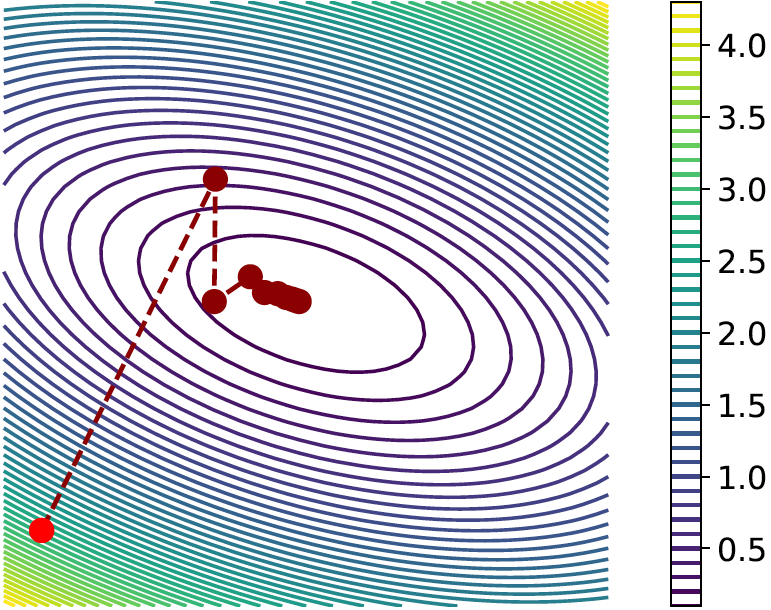
\includegraphics[height=3.5cm]{\toplevelprefix/chapters/appendixA/figs/GD-1.png}
    \hspace{3mm}
    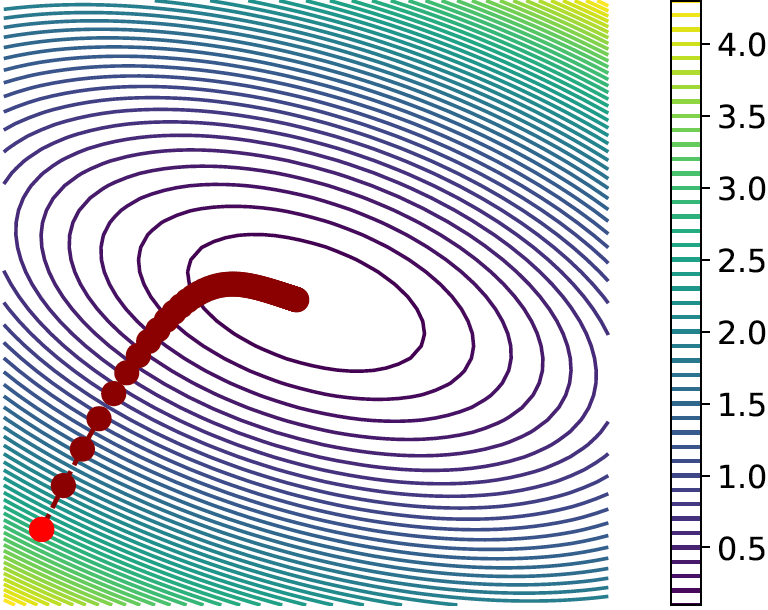
\includegraphics[height=3.5cm]{\toplevelprefix/chapters/appendixA/figs/GD-2.png}
    \hspace{3mm}
    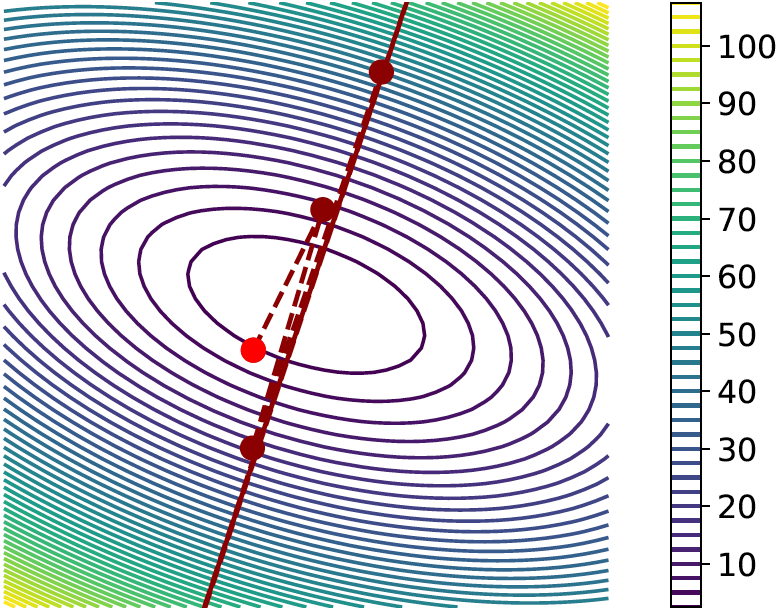
\includegraphics[height=3.5cm]{\toplevelprefix/chapters/appendixA/figs/GD-3.png}
    \caption{步长 \(h\) 对梯度下降法收敛性的影响。}
    \label{fig:step-size}
\end{figure}

所以步长 \(h\) 的选择应该基于函数 \(\cL(\theta_k)\) 的景观(landscape)。理想情况下,为了选择最佳步长 \(h\),我们可以解决以下关于单变量 \(h\) 的优化问题:
\begin{equation}
    h = \argmin_{h\geq 0} \cL(\theta_k - h\nabla \cL(\theta_k)).
\end{equation}
这种选择步长的方法称为\textit{线搜索}(line search)。然而,当函数 \(L(\theta_k)\) 很复杂时,这在训练深度神经网络时通常是如此,这个一维优化问题在梯度下降的每次迭代中都非常难以解决。

那么我们应该如何选择一个合适的步长 \(h\) 呢?一个常见且经典的方法是,基于对函数 \(\cL(\theta)\) 整体景观的一些了解,来获得对当前状态 \(\theta\) 周围局部景观的一个良好近似。

\begin{figure}
    \centering 
    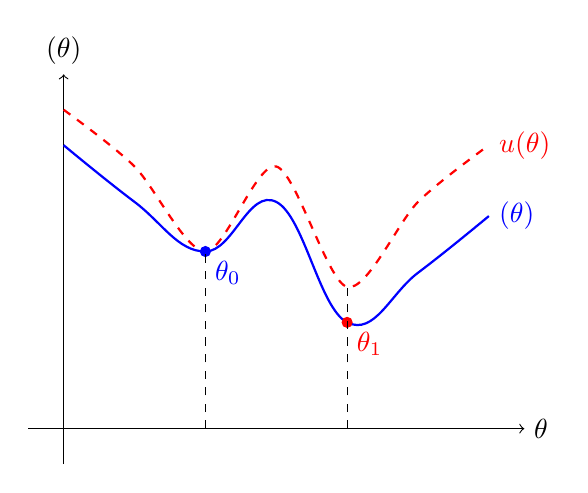
\begin{tikzpicture}[scale=0.9]
        % Axes
        \draw[->] (-0.5,0) -- (6.5,0) node[right] {$\theta$};
        \draw[->] (0,-0.5) -- (0,5) node[above] {$\cL(\theta)$};
        
        % Original function (nonconvex)
        \draw[thick, blue] plot[smooth, tension=0.7] coordinates {
            (0,4) (1,3.2) (2,2.5) (3,3.2) (4,1.5) (5,2.2) (6,3)
        } node[right] {$\cL(\theta)$};
        
        % Upper bound function
        \draw[thick, red, dashed] plot[smooth, tension=0.5] coordinates {
            (0,4.5) (1,3.7) (2,2.5) (3,3.7) (4,2) (5,3.2) (6,4)
        } node[right] {$u(\theta)$};
        
        % Point of equality
        \filldraw[blue] (2,2.5) circle (2pt) node[below right] {$\theta_0$};
        
        % Minimum of upper bound
        \filldraw[red] (4,1.5) circle (2pt) node[below right] {$\theta_1$};
        
        % Vertical lines showing the improvement
        \draw[dashed] (2,0) -- (2,2.5);
        \draw[dashed] (4,0) -- (4,2);
    \end{tikzpicture}
    \caption{\small\textbf{主化-最小化(Majorization-Minimization)方案与直观解释。} 一个函数 \(\cL \colon \Theta \to \R\) 有一个全局上界 \(u \colon \Theta \to \R\),它与 \(\cL\) 至少在一个点 \(\theta_{0}\) 相切。那么,找到最小化 \(u\) 的 \(\theta_{1}\) 将会改进 \(\cL\) 的值,从 \(\cL(\theta_{0})\) 变得更小。注意,对于局部上界也可以证明类似的结果。}
    \label{fig:majorization_minimization}
\end{figure}

函数 \(\cL(\theta)\) 景观的常见条件包括:
\begin{itemize}
    \item \(\alpha\)-强凸性。回顾一下,如果 \(\cL\) 的图像位于一个斜率为 \(\alpha\) 的全局二次下界之上,那么 \(\cL\) 是\textit{\(\alpha\)-强凸}的,即
    \begin{equation}
        \cL(\theta) \geq l_{\theta_{0}, \alpha}(\theta) \doteq \cL(\theta_{0}) + \ip{\nabla \cL(\theta_{0})}{\theta - \theta_{0}} + \frac{\alpha}{2}\norm{\theta - \theta_{0}}_{2}^{2}
    \end{equation}
    对于任何“基点” \(\theta_{0}\) 都成立。如果 \(\cL\) 是 \(0\)-强凸的,即其图像位于其切线之上,我们称 \(\cL\) 是\textit{凸}的。很容易证明(作为练习)强凸函数有唯一的全局最小值。另一个重要的事实是(作为练习证明),\(\alpha\)-强凸的二次可微函数 \(\cL\) 具有(对称的)海森矩阵 \(\nabla^{2}\cL\),其最小特征值 \(\geq \alpha\)。对于 \(\alpha > 0\),这意味着海森矩阵是半正定的,而对于 \(\alpha = 0\)(即 \(\cL\) 是凸的),这意味着海森矩阵是半正定的。
    \item \(\beta\)-梯度利普希茨(也称为 \(\beta\)-光滑性)。回顾一下,如果 \(\nabla \cL\) 存在且是 \(\beta\)-利普希茨的,那么 \(\cL\) 具有\textit{\(\beta\)-梯度利普希茨}性质,即
    \begin{equation}
        \norm{\nabla \cL(\theta) - \nabla \cL(\theta_{0})}_{2} \leq \beta \norm{\theta - \theta_{0}}_{2}.
    \end{equation}
    对于任何“基点” \(\theta_{0}\) 都成立。很容易证明(作为练习),这等价于 \(\cL\) 有一个斜率为 \(\beta\) 的全局二次上界,即
    \begin{equation}
        \cL(\theta) \leq u_{\theta_{0}, \beta}(\theta) \doteq \cL(\theta_{0}) + \ip{\nabla \cL(\theta_{0})}{\theta - \theta_{0}} + \frac{\beta}{2}\norm{\theta - \theta_{0}}_{2}^{2}.
    \end{equation}
    对于任何“基点” \(\theta_{0}\) 都成立。另一个重要的事实是(作为练习证明),具有 \(\beta\)-梯度利普希茨性质的二次可微凸函数,其(对称的)海森矩阵 \(\nabla^{2}\cL\) 的最大特征值 \(\leq \beta\)。
\end{itemize}
首先,让我们假设 \(\cL\) 具有 \(\beta\)-梯度利普希茨性质(但不一定甚至是凸的)。我们将借此机会介绍一个常见的优化主题:\textit{为了最小化 \(\cL\),我们可以最小化 \(L\) 的一个上界},这由\Cref{fig:majorization_minimization}中可视化的以下引理来证明。
\begin{lemma}[主化-最小化]\label{lem:majorization_minimization}
    假设 \(u \colon \Theta \to \R\) 是 \(\cL\) 的一个全局上界,即对所有 \(\theta \in \Theta\),有 \(\cL(\theta) \leq u(\theta)\)。假设它们在 \(\theta_{0}\) 处相等,即 \(\cL(\theta_{0}) = u(\theta_{0})\)。那么
    \begin{equation}
        \theta_{1} \in \argmin_{\theta \in \Theta}u(\theta) \implies \cL(\theta_{1}) \leq u(\theta_{1}) \leq u(\theta_{0}) = \cL(\theta_{0}).
    \end{equation}
\end{lemma}

我们将使用这个引理来表明,我们可以利用梯度利普希茨性质来确保每个梯度步骤不会使 \(\cL\) 的值恶化。确实,在每个基点 \(\theta_{0}\) 处,我们有 \(u_{\theta_{0}, \beta}\) 是 \(\cL\) 的一个全局上界,并且 \(u_{\theta_{0}, \beta}(\theta_{0}) = \cL(\theta_{0})\)。因此根据\Cref{lem:majorization_minimization}
\begin{equation}
    \text{如果 \(\theta\) 最小化 \(u_{\theta_{0}, \beta}\),那么} \quad \cL(\theta) \leq u_{\theta_{0}, \beta}(\theta) \leq u_{\theta_{0}, \beta}(\theta_{0}) = \cL(\theta_{0}).
\end{equation}
这启发我们,当从 \(\theta_{k}\) 寻找更新以获得 \(\theta_{k + 1}\) 时,我们可以转而最小化上界 \(u_{\theta_{k}, \beta}\) 关于 \(\theta\) 的值,并将其设为 \(\theta_{k + 1}\)。通过最小化 \(u_{\theta_{k}, \beta}\)(作为练习证明),我们得到
\begin{equation}\label{eq:GD}
    \theta_{k + 1} = \theta_{k} - \frac{1}{\beta}\nabla \cL(\theta_{k}) \implies \cL(\theta_{k + 1}) \leq \cL(\theta_{k}).
\end{equation}
这意味着步长 \(h = 1/\beta\) 是一个可用的学习率,但这并未提供收敛速率,也未证明 \(L(\theta_{k})\) 确实收敛到 \(\min_{\theta}\cL(\theta)\)。这需要更严谨的论证,我们现在就来进行。

现在,让我们假设 \(\cL\) 是 \(\alpha\)-强凸的,具有 \(\beta\)-梯度利普希茨性质,并且有全局最优解 \(\theta^{\star}\)。我们将证明 \(\theta_{k}\) 将直接收敛到唯一的全局最优解 \(\theta^{\star}\),这是一种非常强的收敛形式。具体来说,我们将利用 \(\cL\) 的强凸性和梯度的利普希茨性质来界定 \(\norm{\theta^{\star} - \theta_{k}}_{2}\),即考察 \(\theta_{k}\) 周围的邻域:\footnote{在这个证明中,\(\beta\)-梯度利普希茨的调用步骤有点不那么直接。我们也把这一步作为练习,提示是将 \(\theta = \theta_{0} - h\nabla \cL(\theta_{0})\) 代入梯度利普希茨恒等式。}
\begin{align}
    \norm{\theta^{\star} - \theta_{k + 1}}_{2}^{2}
    &\leq \norm{\theta^{\star} - \theta_{k} + h\nabla \cL(\theta_{k})}_{2}^{2} \\ 
    &= \norm{\theta^{\star} - \theta_{k}}_{2}^{2} + 2h\ip{\nabla \cL(\theta_{k})}{\theta^{\star} - \theta_{k}} + h^{2}\norm{\nabla \cL(\theta_{k})}_{2}^{2} \\ 
    &\leq \norm{\theta^{\star} - \theta_{k}}_{2}^{2} + 2h\bp{\cL(\theta^{\star}) - \cL(\theta_{k}) - \frac{\alpha}{2}\norm{\theta^{\star} - \theta_{k}}_{2}^{2}} + h^{2}\norm{\nabla \cL(\theta_{k})}_{2}^{2} \quad \text{(\(\alpha\)-强凸)} \\
    &= \bp{1 - \alpha h}\norm{\theta^{\star} - \theta_{k}}_{2}^{2} + 2h(\cL(\theta^{\star}) - L(\theta_{k})) + h^{2}\norm{\nabla \cL(\theta_{k})}_{2}^{2} \\
    &\leq \bp{1 - \alpha h}\norm{\theta^{\star} - \theta_{k}}_{2}^{2} + 2h(\cL(\theta^{k}) - \cL(\theta^{\star})) + 2h^{2}\beta(\cL(\theta_{k}) - \cL(\theta^{\star})) \quad \text{(\(\beta\)-梯度利普希茨)} \\
    &= \bp{1 - \alpha h}\norm{\theta^{\star} - \theta_{k}}_{2}^{2} - 2h(1 - \beta h)(\cL(\theta_{k}) - \cL(\theta^{\star})).
\end{align}
为了确保梯度下降迭代取得进展,我们必须选择步长使得 \(1 - \beta h \geq 0\),即 \(h \leq 1/\beta\)。如果满足这个设置,那么
\begin{align}
    \norm{\theta^{\star} - \theta_{k + 1}}_{2}^{2} 
    &\leq (1 - \alpha h)\norm{\theta^{\star} - \theta_{k}}_{2}^{2} \leq (1 - \alpha h)^{2}\norm{\theta^{\star} - \theta_{k - 1}}_{2}^{2} \leq \cdots \\ 
    &\leq (1 - \alpha h)^{k + 1}\norm{\theta^{\star} - \theta_{0}}_{2}^{2}.
\end{align}
为了最小化右侧,我们可以设置 \(h = 1/\beta\),从而得到
\begin{equation}
    \norm{\theta^{\star} - \theta_{k + 1}}_{2}^{2} \leq (1 - \alpha/\beta)^{k + 1}\norm{\theta^{\star} - \theta_{0}}_{2}^{2},
\end{equation}
这表明误差以指数形式衰减,收敛到全局最优点。注意,这里我们使用了一个收敛速率来获得一个有利的\textit{步长} \(h = 1/\beta\)。这个模式将在本节中再次出现。

我们以一个警示结束本节:学习全局最优点(通常)是不切实际的困难。在某些条件下,我们可以确保梯度下降的迭代收敛到一个\textit{局部最优点}。此外,在更宽松的条件下,我们可以确保\textit{局部}收敛,即如果序列在离最优点足够近的地方初始化,迭代会收敛到一个(全局或局部)最优点。

% \DP{TODO: Exercise based on convergence proof for PL condition + Lipschitz gradient.}

\subsection{针对病态问题的预条件梯度下降法}

% \DP{I realized after writing this section that the second-order approximation is not needed for any other section (I thought proximal gradient used second-order approximation but it only needs Lipschitz gradient upper bound). However, I think PSGD is very useful in practice. @YM up to you whether to keep this section.}
% \yima{I think this is ok for now.}

\begin{figure}
    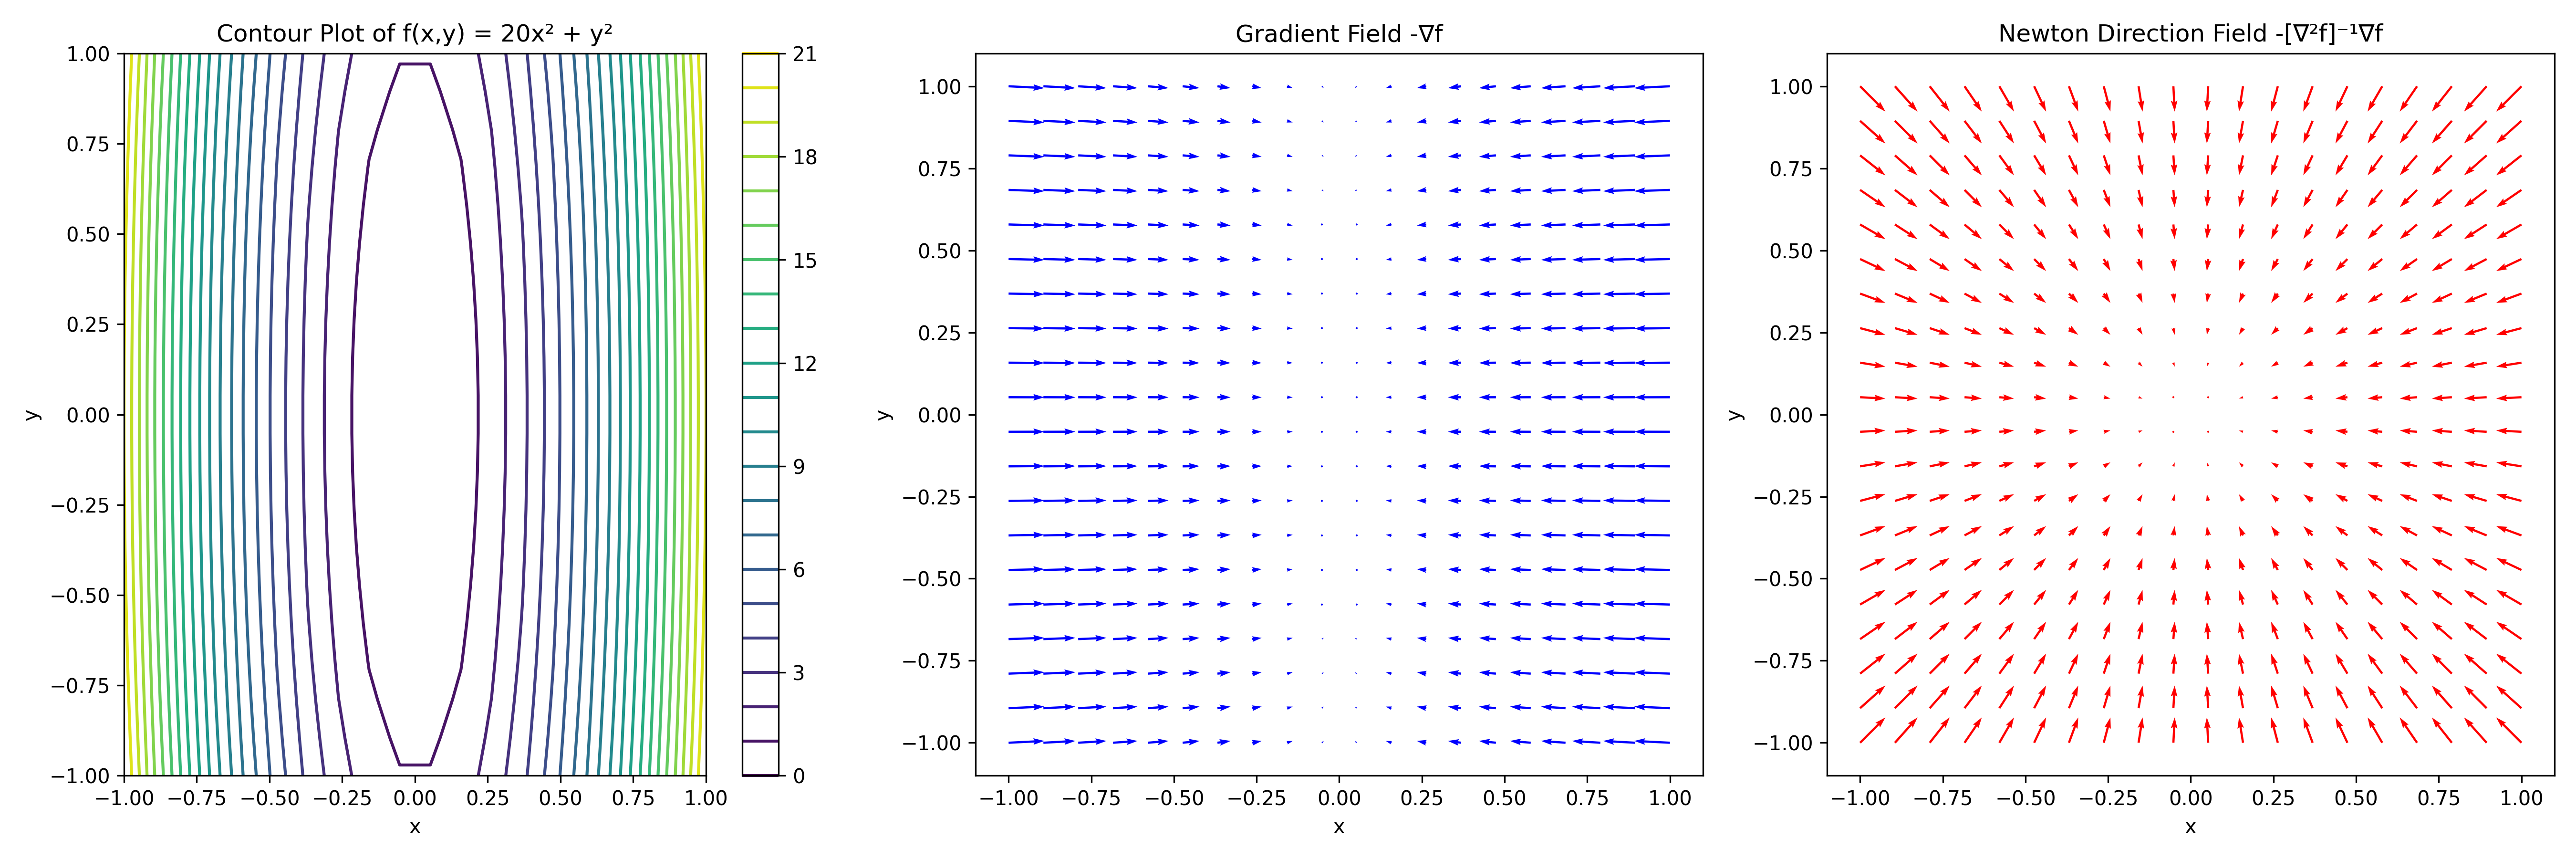
\includegraphics[width=\textwidth]{\toplevelprefix/chapters/appendixA/figs/hessian_geometry.png}
    \caption{\small\textbf{负梯度 \(-\nabla \cL_{\lambda}\) 与预条件(牛顿法步长)向量场 \(-[\nabla^{2}\cL_{\lambda}]^{-1}[\nabla \cL_{\lambda}]\)},其中 \(\lambda = 19\)。在空间的某个区域,沿着负梯度向量场在寻找最小值方面进展甚微,但在所有情况下,遵循牛顿法向量场都能以相同的速度朝最优点前进,因为梯度被白化了。由于这里的海森矩阵是对角的,自适应学习率算法(例如稍后将讨论的Adam)可以取得与牛顿法相似的进展,但一个非轴对齐的海森矩阵甚至可能阻碍Adam快速成功。}
    \label{fig:hessian_geometry}
\end{figure}

\subsubsection{牛顿法}

对于一些光滑问题和强凸问题,梯度下降法的表现仍然相当差。例如,令 \(\lambda \geq 0\),并令 \(\cL_{\lambda} \colon \R^{2} \to \R\) 的形式为
\begin{equation}
    \cL_{\lambda}(\theta) = \cL_{\lambda}\rp{\mat{\theta_{1} \\ \theta_{2}}} \doteq \frac{1}{2}\bc{(1 + \lambda) \theta_{1}^{2} + \theta_{2}^{2}} = \frac{1}{2}\theta^{\top}\mat{1 + \lambda & 0 \\ 0 & 1}\theta.
\end{equation}
这个问题是 \(1\)-强凸的,并且具有 \((1 + \lambda)\)-梯度利普希茨性质。其收敛速率是几何级的,速率为 \(1 - 1/(1 + \lambda)\)。对于大的 \(\lambda\),这个速度仍然不是很快。在本节中,我们将介绍一类可以成功优化这类病态函数的优化问题。

关键在于目标的\textit{曲率},它由海森矩阵给出。假设(作为一个反事实的假设)我们有一个\textit{二阶}神谕机,它允许我们计算 \(\cL(\theta)\)、\(\nabla \cL(\theta)\) 和 \(\nabla^{2}\cL(\theta)\)。那么,我们不必选择一个下降方向 \(\vv\) 来优化 \(\theta\) 周围的一阶泰勒展开,而是可以优化二阶泰勒展开。直观上,这将允许我们将曲率信息纳入更新中。

让我们来进行这个计算。 \(\cL(\theta + h\vv)\) 在 \(h = 0\) 附近的二阶泰勒展开是
\begin{equation}
    \cL(\theta + h\vv) = \cL(\theta) + h\ip{\nabla \cL(\theta)}{\vv} + \frac{1}{2}h^{2}\ip{[\nabla^{2}\cL(\theta)]\vv}{\vv} + o(h^{2}).
\end{equation}
然后我们可以计算下降方向:
\begin{align}
    \argmin_{\substack{\vv \in \R^{n} \\ \norm{\vv}_{2} = 1}}\bs{\cL(\theta) + h\ip{\nabla \cL(\theta)}{\vv} + \frac{1}{2}h^{2}\ip{[\nabla^{2}\cL(\theta)]\vv}{\vv}} 
    &= \argmin_{\substack{\vv \in \R^{n} \\ \norm{\vv}_{2} = 1}}\bs{\ip{\nabla \cL(\theta)}{\vv} + \frac{1}{2}h\ip{[\nabla^{2}\cL(\theta)]\vv}{\vv}}.
\end{align}
由于约束 \(\norm{\vv}_{2} = 1\),这个优化问题有点难以解决。但在实践中,我们从不归一化下降方向 \(\vv\),而是使用步长 \(h\) 来控制更新的大小。所以让我们直接在所有向量 \(\vv \in \R^{n}\) 上解决上述问题:\footnote{如果 \(\nabla^{2}\cL(\theta)\) 不可逆,那么我们可以用 \(\nabla^{2}\cL(\theta)\) 的摩尔-彭若斯伪逆来代替 \([\nabla^{2}\cL(\theta)]^{-1}\)。}
\begin{equation}
    \argmin_{\vv \in \R^{n}}\bs{\ip{\nabla \cL(\theta)}{\vv} + \frac{1}{2}h\ip{[\nabla^{2}\cL(\theta)]\vv}{\vv}} = -\frac{1}{h}[\nabla^{2}\cL(\theta)]^{-1}[\nabla \cL(\theta)].
\end{equation}
因此,我们可以使用最速下降迭代
\begin{equation}
    \theta_{k + 1} = \theta_{k} - [\nabla^{2}\cL(\theta_{k})]^{-1}[\nabla \cL(\theta_{k})],
\end{equation}
(这就是著名的\textit{牛顿法}),或者
\begin{equation}
    \theta_{k + 1} = \theta_{k} - h[\nabla^{2}\cL(\theta_{k})]^{-1}[\nabla \cL(\theta_{k})],
\end{equation}
(这被称为\textit{欠阻尼牛顿法})。由于二阶二次函数 \(\cL_{\lambda}\) 等于其二阶泰勒展开,如果我们运行牛顿法\textit{一步},无论 \(\lambda\) 有多大,我们都将\textit{一步}达到全局最小值。\Cref{fig:hessian_geometry} 给出了一些关于病态函数以及梯度步长与牛顿步长的直观解释。

\subsubsection{PGD}

在实践中,我们\textit{没有}一个二阶神谕机来让我们计算 \(\nabla^{2}\cL(\theta)\)。相反,我们可以尝试在从 \(\theta_{k}\) 更新到 \(\theta_{k + 1}\) 的同时,\textit{学习它的一个近似}。

我们如何学习它的近似呢?我们将找到海森矩阵的逆满足的一些方程,然后尝试更新我们的近似,使其满足这些方程。具体来说,取 \(\nabla \cL(\theta + \delta_{\theta})\) 在点 \(\theta\) 的泰勒级数,我们得到
\begin{equation}
    \underbrace{\nabla L(\theta + \delta_{\theta}) - \nabla \cL(\theta)}_{\doteq \delta_{\vg}} = [\nabla^{2} \cL(\theta)]\delta_{\theta} + o(\norm{\delta_{\theta}}_{2}).
\end{equation}
在这种情况下,我们有
\begin{equation}
    \delta_{\vg} \approx [\nabla^{2}\cL(\theta)]\delta_{\theta} \implies \delta_{\theta} \approx [\nabla^{2}\cL(\theta)]^{-1}\delta_{\vg}
\end{equation}
我们现在可以尝试学习一个对称半正定的预条件子 \(P \in \R^{n \times n}\),使得
\begin{equation}
    \delta_{\theta} \approx P\delta_{\vg},
\end{equation}
并在每次迭代中与 \(\theta_{k}\) 一起更新它。具体来说,我们有\textit{PSGD}迭代
\begin{align}
    P_{k}
    &= \mathrm{PreconditionerUpdate}(P_{k - 1}; \theta_{k}, \nabla \cL(\theta_{k})) \\ 
    \theta_{k + 1}
    &= \theta_{k} - hP_{k}\nabla \cL(\theta_{k}).
\end{align}
这个更新有两个问题:我们如何使用 \(P\)(因为我们已经说过我们不能存储一个 \(n \times n\) 的矩阵),以及我们如何在每次迭代中\textit{更新} \(P\)?答案是密切相关的;我们永远无法在计算机内存中实体化 \(P\),但我们可以用低秩分解(或类似的方法,如特别适用于深度神经网络形式的\textit{克罗内克分解})来表示它。然后,预条件子更新步骤被设计为利用预条件子表示的结构。

我们以一个警示结束本小节:在深度学习中,例如,\(\cL\) 不是一个凸函数,因此牛顿法(及其近似)没有意义。在这种情况下,我们关注牛顿法在凸函数上的几何直观,比如说从\Cref{fig:hessian_geometry}中:逆海森矩阵\textit{白化}了梯度。因此,我们不必使用一个近似海森矩阵的预条件子,而是可以调整上述过程来学习一个更通用的梯度白化变换。这是PSGD原始提议 \cite{li2017preconditioned} 背后的思想,其中包含了更多关于如何存储和更新预条件子的信息,以及更现代的优化器如Muon \cite{liu2025muon}。


\subsection{针对非光滑问题的近端梯度下降法}\label{subsec:pgd}

然而,即使在非常简单的玩具问题中,例如LASSO或字典学习,问题也不再是强凸的,而仅仅是凸的,并且目标函数也不再仅仅是光滑的,而是光滑函数和非光滑正则化项(如 \(\ell^{1}\) 范数)的和。这类问题通过\textit{近端优化算法}来解决,这些算法将最速下降法推广到非光滑目标函数。

形式上,我们说
\begin{equation}
    \cL(\theta) \doteq \cS(\theta) + \cR(\theta)
\end{equation}
其中 \(\cS\) 是光滑的,比如说具有 \(\beta\)-梯度利普希茨性质,而 \(\cR\) 是非光滑的(即粗糙的)。近端梯度算法推广了最速下降算法,通过使用主化-最小化框架(即 \Cref{lem:majorization_minimization})和一个不同的全局上界。具体来说,我们通过提出以下问题来构造这样一个上界:如果我们取 \(\cS\) 的梯度利普希茨上界但\textit{保持 \(\cR\) 不变}会怎么样?也就是说,我们有
\begin{equation}
    \cL(\theta_{1}) = \cS(\theta_{1}) + \cR(\theta_{1}) \leq u_{\theta_{0}, \beta}(\theta_{1}) \doteq \cS(\theta_{0}) + \ip{\nabla \cS(\theta_{0})}{\theta_{1} - \theta_{0}} + \frac{\beta}{2}\norm{\theta_{1} - \theta_{0}}_{2}^{2} + \cR(\theta_{1}).
\end{equation}
注意(作为练习证明)
\begin{equation}
    \argmin_{\theta_{1}}u_{\theta_{0}, \beta}(\theta_{1}) = \argmin_{\theta_{1}}\bs{\frac{\beta}{2}\norm*{\theta_{1} - \bp{\theta_{0} - \frac{1}{\beta}\nabla \cS(\theta_{0})}}_{2}^{2} + \cR(\theta_{1})}.
\end{equation}
现在,如果我们试图最小化上界 \(u_{\theta_{0}, \beta}\),我们选择的 \(\theta_{1}\) 将会:
\begin{itemize}
    \item 接近梯度更新 \(\theta_{0} - \frac{1}{\beta}\nabla \cS(\theta_{0})\);
    \item 具有较小的正则化项 \(\cR(\theta_{1})\) 的值
\end{itemize}
并根据光滑性参数 \(\beta\) 来权衡这些属性。因此,我们定义近端算子
\begin{equation}
    \prox_{h, \cR}(\theta) \doteq \argmin_{\theta_{1}}\bs{\frac{1}{2h}\norm{\theta_{1} - \theta}_{2}^{2} + \cR(\theta)}.
\end{equation}
然后,我们可以定义\textit{近端梯度下降}迭代,它在每次迭代中最小化上界 \(u_{\theta_{k}, h^{-1}}\),即
\begin{equation}
    \theta_{k + 1} = \prox_{h, \cR}(\theta_{k} - h\nabla \cS(\theta_{k})).
\end{equation}
当 \(h \leq 1/\beta\) 时,可以证明收敛性,但我们不在本节中给出任何证明。

一个遗留问题是:我们如何计算近端算子?乍一看,我们似乎只是用一个棘手的最小化问题换了另一个。由于到目前为止我们没有对 \(\cR\) 做任何假设,这个框架即使在 \(\cR\) 是一个非常复杂的函数(比如一个神经网络损失)时也适用,这将要求我们为了计算一个单一的近端算子而解决一个神经网络训练问题。然而,在实践中,对于简单的正则化项 \(\cR\),比如我们在本手稿中使用的那些,存在易于计算甚至有闭式解的近端算子。下面我们给出几个例子(证明作为练习)。

\begin{example}\label{example:prox-of-characteristic-function}
    令 \(\Gamma \subseteq \Theta\) 是一个集合,令 \(\chi_{\Gamma}\) 是 \(\Gamma\) 上的特征函数,即
    \begin{equation}
        \chi_{\Gamma}(\theta) \doteq \casework{0, & \text{若}\ \theta \in \Gamma \\ +\infty, & \text{若}\ \theta \notin \Gamma.}
    \end{equation}
    那么 \(\chi_{\Gamma}\) 的近端算子是一个投影,即
    \begin{equation}
        \prox_{h, \chi_{\Gamma}}(\theta) = \argmin_{\theta_{1} \in \Gamma}\frac{1}{2}\norm{\theta_{1} - \theta}_{2}^{2} = \argmin_{\theta_{1} \in \Gamma}\norm{\theta_{1} - \theta}_{2}.
    \end{equation}
\end{example}

\begin{example}\label{example:prox-of-l1}
    \(\ell^{1}\) 范数有一个执行软阈值操作的近端算子:
    \begin{equation}
        S_{h}(\theta) \doteq \prox_{h, \lambda \norm{\cdot}_{1}}(\theta) = \argmin_{\theta_{1}}\bs{\frac{1}{2h}\norm{\theta_{1} - \theta}_{2}^{2} + \lambda\norm{\theta}_{1}}
    \end{equation}
    那么 \(S_{h}(\theta)\) 定义为
    \begin{equation}
        S_{h}(\theta)_{i} = \casework{\theta_{i} - h\lambda, & \text{若}\ \theta_{i} \geq h\lambda \\ 0, & \text{若}\ \theta_{i} \in [-h\lambda, h\lambda] \\ \theta_{i} + h\lambda, & \text{若}\ \theta_{i} \leq -h\lambda} = \casework{\max\{\abs{\theta_{i}} - h\lambda, 0\}\sign(\theta_{i}), & \text{若}\ \abs{\theta_{i}} \geq h\lambda \\ 0, & \text{若}\ \abs{\theta_{i}} < h\lambda.}
    \end{equation}
    目标函数的光滑部分是最小二乘,非光滑部分是 \(\ell^{1}\) 范数的近端梯度操作(因此使用这个软阈值近端算子)被称为迭代收缩阈值算法(ISTA)。
\end{example}

\begin{example}\label{example:prox-of-nonnegative-l1}
    在\Cref{ch:representation}中,我们使用一个对应于 \(\ell^{1}\) 范数加上正象限 \(\R_{+}^{n} \doteq \{\vx \in \R^{n} \colon x_{i} \geq 0\ \forall i\}\) 的特征函数的近端算子,即
    \begin{equation}
        T_{h}(\theta) \doteq \prox_{h, \lambda\norm{\cdot}_{1} + \chi_{\R_{+}^{n}}}(\theta) = \argmin_{\theta_{1} \in \R_{+}^{n}}\bs{\frac{1}{2h}\norm{\theta_{1} - \theta}_{2}^{2} + \lambda\norm{\theta}_{1}},
    \end{equation}
    那么 \(T_{h}\) 定义为
    \begin{equation}
        T_{h}(\theta)_{i} \doteq \max\{\theta_{i} - h\lambda, 0\}.
    \end{equation}
    这个近端算子产生了在\Cref{ch:representation}及以后章节中调用的非负ISTA。
\end{example}


% \DP{Optional: @SB want to put some stuff in about learning a prox}

\subsection{针对大规模问题的随机梯度下降法}

% \yima{Maybe here introducing stochastic gradient descent for the case when $f(\x)$ needs to be estimated as an expectation $f(\x) = \mathbb{E}_{\boldsymbol{w}}(f(\x, \boldsymbol{w})$ samples of another random variable $\boldsymbol{w}$, as in the case of training a neural networks with an expected loss over a batch of samples. Druv or Sam? One problem is that here we use $\x$ as the optimization variable but in the deep networks below we use $\bm(\theta)$... and $\x$ for the samples. Make notation better later!}

在深度学习中,目标函数 \(\cL\) 通常无法精确计算,而是在每个优化步骤中使用有限样本(例如,使用一个小批量)进行\textit{估计}。一个常见的建模这种情况的方法是定义一个\textit{随机损失函数} \(\cL_{\omega}(\theta)\),其中 \(\omega\) 是某种“随机性来源”。例如,\(\omega\) 可以包含一个批次中用于计算损失的样本索引。然后,我们希望在给定一个\textit{随机一阶神谕机}的情况下,最小化 \(\cL(\theta) \doteq \Ex_{\omega}[\cL_{\omega}(\theta)]\) 关于 \(\theta\) 的值:给定 \(\theta\),我们可以采样 \(\omega\) 并计算 \(\cL_{\omega}(\theta)\) 和 \(\nabla_{\theta}\cL_{\omega}(\theta)\)。这个最小化问题被称为\textit{随机优化问题}。

基本的随机一阶算法是\textit{随机梯度下降}:在每次迭代 \(k\) 中,我们采样 \(\omega_{k}\),定义 \(\cL_{k} \doteq \cL_{\omega_{k}}\),并在 \(\cL_{k}\) 上执行一个梯度步骤,即
\begin{equation}
    \theta_{k + 1} = \theta_{k} - h\nabla \cL_{k}(\theta_{k}).
\end{equation}
然而,即使对于非常简单的问题,我们也不能期望得到与梯度下降中相同的收敛类型。例如,假设 \(\omega \in \{1, \dots, m\}\) 有 \(m\) 个可能的值,它以等概率取值,并且有 \(m\) 个可能的目标 \(\xi_{1}, \dots, \xi_{m}\),使得损失函数 \(\cL_{\omega}\) 是
\begin{equation}
    \cL_{\omega}(\theta) \doteq \frac{1}{2}\norm{\theta - \xi_{\omega}}_{2}^{2}.
\end{equation}
那么 \(\argmin_{\theta}\Ex[\cL_{\omega}(\theta)] = \frac{1}{m}\sum_{i = 1}\xi_{i}\),但随机梯度下降可能会在全局最优点附近“弹跳”,而不会收敛,如\Cref{fig:sgd_nonconvergence}所示。

\begin{figure}
    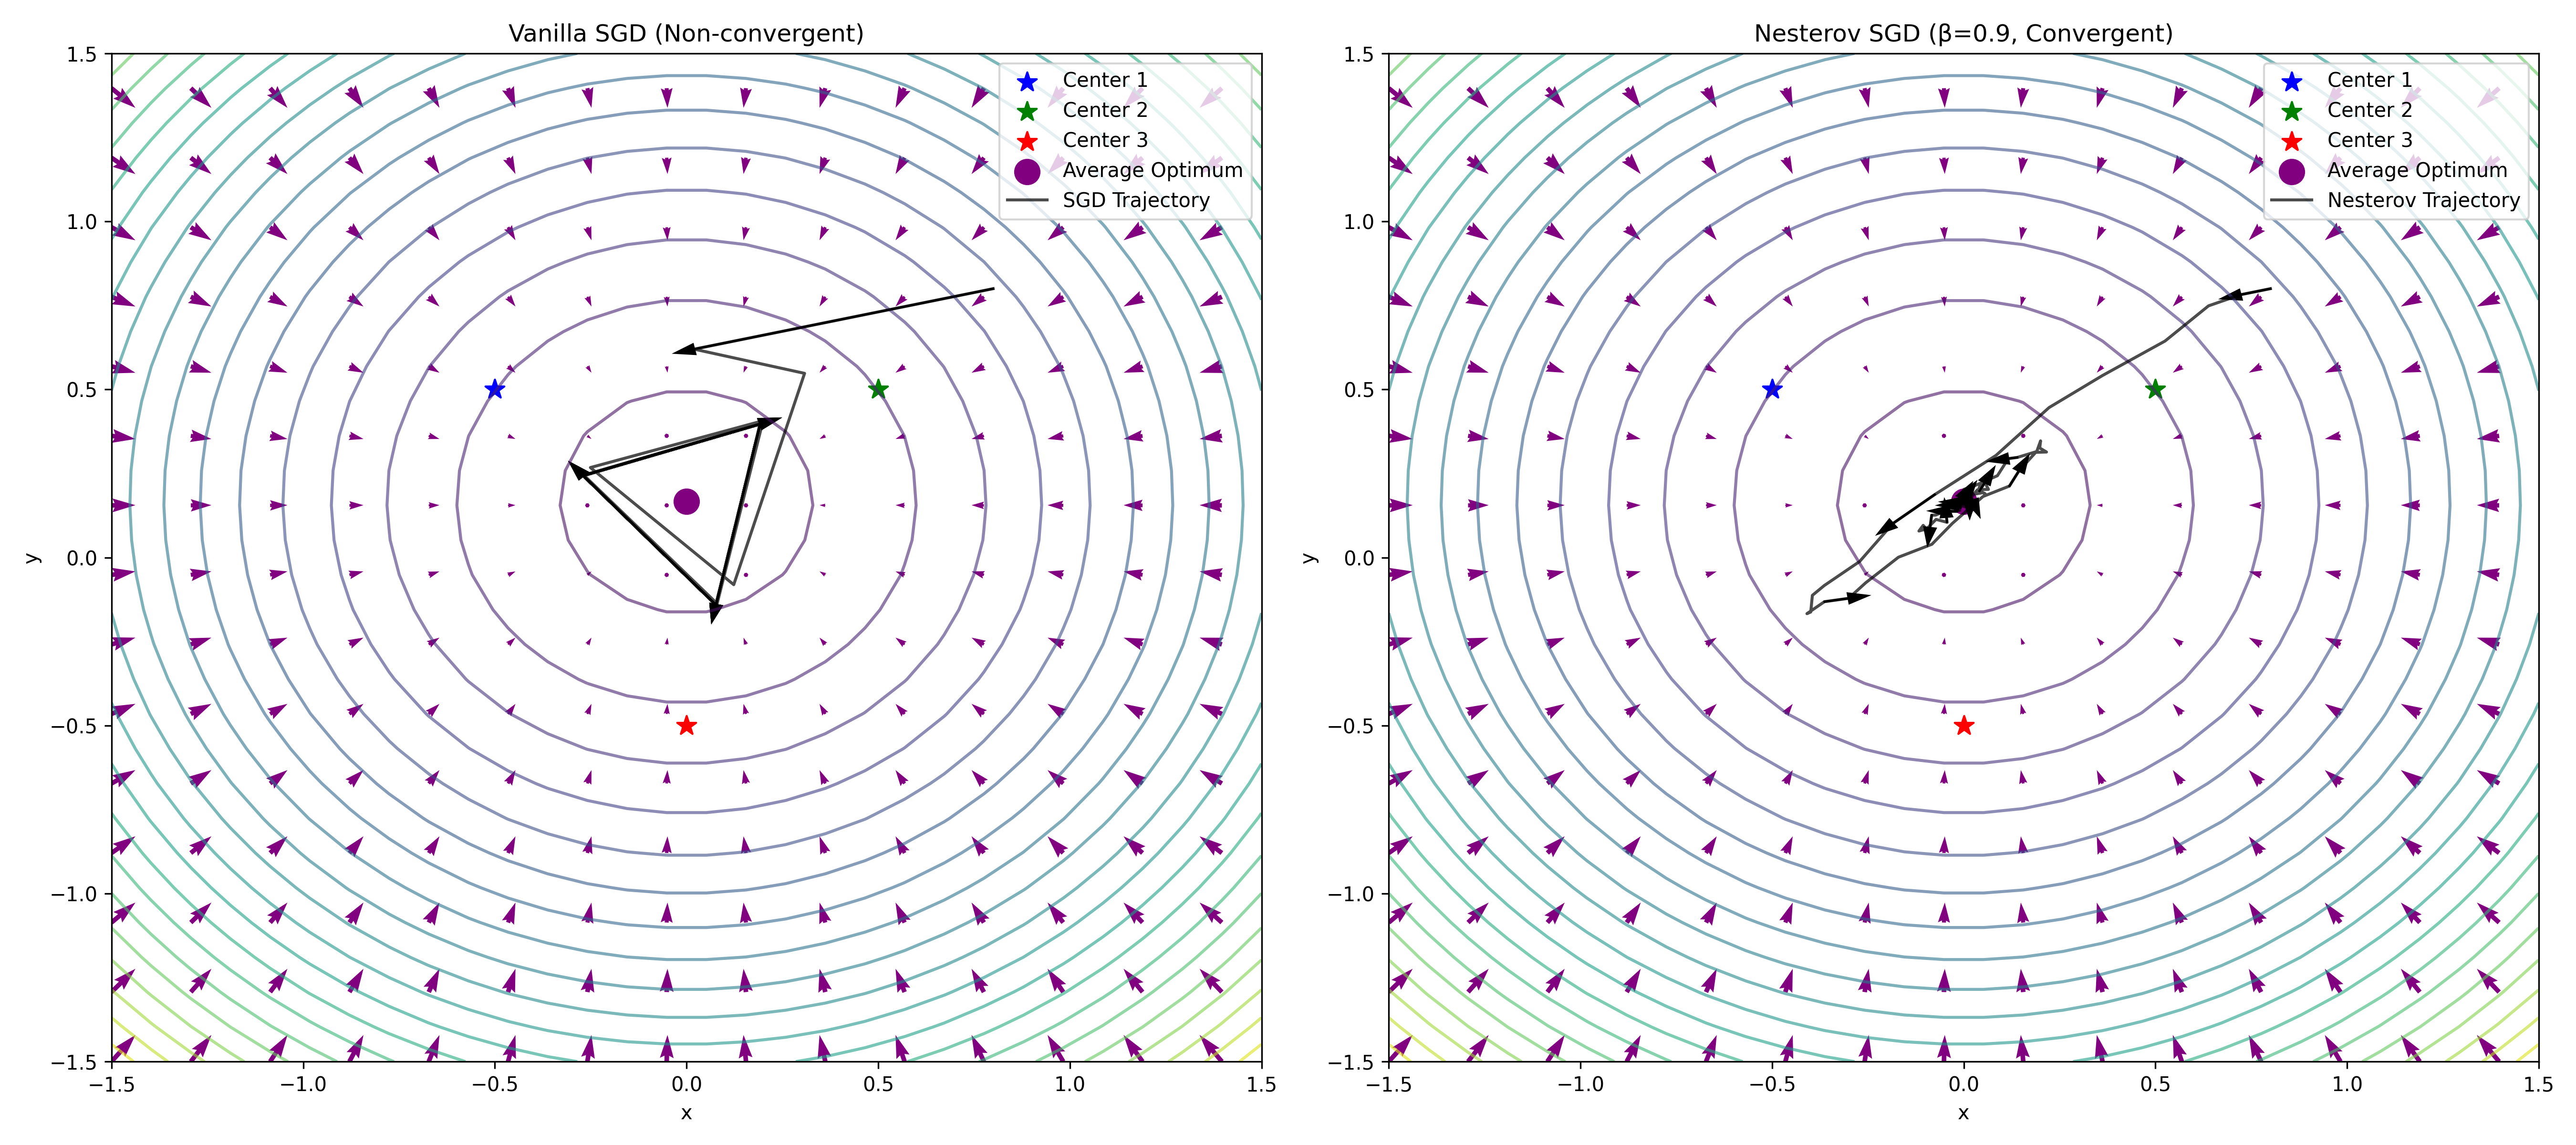
\includegraphics[width=\textwidth]{\toplevelprefix/chapters/appendixA/figs/sgd_vs_nesterov.png}
    \centering 
    \caption{\small\textbf{即使对于非常良性的目标,随机梯度下降也可能不收敛,但Nesterov梯度会收敛。} 即使对于简单的二次目标函数,随机梯度下降的迭代也可能在全局最优点附近弹跳,而Nesterov梯度则会对齐以指向最优值。}
    \label{fig:sgd_nonconvergence}
\end{figure}

为了解决这个问题,我们可以随时间平均参数 \(\theta_{k}\) 或平均梯度 \(\nabla \cL_{k}(\theta_{k})\)。如果我们平均参数 \(\theta_{k}\),那么(以\Cref{fig:sgd_nonconvergence}为心智模型)弹跳问题就直接不可能发生,因为平均迭代点会越来越接近中心。因此,大多数理论收敛性证明都考虑平均迭代点 \(\frac{1}{k}\sum_{i = 0}^{k}\theta_{i}\) 向全局最小值的收敛。如果我们平均梯度,我们最终会学到一个平均梯度 \(\frac{1}{k}\sum_{i = 0}^{k}\nabla \cL_{k}(\theta_{k})\),它在每次迭代中变化不大,因此不会弹跳。

在实践中,我们不使用算术平均,而是对参数(这被称为\textit{Polyak动量})或梯度(这被称为\textit{Nesterov动量})进行\textit{指数移动平均}(EMA)。Nesterov动量更受欢迎,我们在这里研究它。

带有Nesterov动量的随机梯度下降迭代如下:
\begin{align}
    \vg_{k}
    &= \beta\vg_{k - 1} + (1 - \beta)\nabla \cL_{k}(\theta_{k}) \\ 
    \theta_{k + 1}
    &= \theta_{k} - h\vg_{k}.
\end{align}
我们不进行收敛性证明(可参见\cite{garrigos2023handbook}的第7章作为例子)。然而,Nesterov动量可以轻松处理我们在\Cref{fig:sgd_nonconvergence}中的玩具案例(见右图):它停止了弹跳并最终收敛到全局最优点。

我们以一个警示结束:可以证明,对于某些参数设置,Polyak动量和Nesterov动量是等价的。那么,也可以证明,带有衰减学习率策略(即学习率 \(h\) 依赖于迭代 \(k\),且其极限为 \(h_{k} \to 0\) 当 \(k \to \infty\) 时)的朴素SGD(或PSGD)可以模仿动量的效果。具体来说,\cite{defazio2023optimal} 表明,如果SGD算法持续 \(K\) 次迭代,梯度范数有界 \(\norm{\nabla \cL(\theta_{k})}_{2} \leq G\),并且我们定义 \(D \doteq \norm{\theta_{0} - \theta^{\star}}_{2}\),那么朴素SGD迭代 \(\theta_{k}\) 满足速率 \(\Ex[\cL(\theta_{k}) - \cL(\theta^{\star})] \leq DG/\sqrt{K}\) --- 但前提是学习率 \(h_{k} = (D/[G\sqrt{K}])(1 - k/K)\) 随时间\textit{线性}衰减。这与实践中使用的学习率策略相匹配。事实上,令人惊讶的是,这样一个凸优化理论可以预测深度网络中的许多经验现象 \cite{schaipp2025surprising},尽管深度学习优化在最坏情况下是高度非凸和非光滑的。目前尚不清楚为什么会这样。


\subsection{集大成者:Adam}

梯度下降方案提出了以下形式的迭代
\begin{equation}
    \theta_{k + 1} = \theta_{k} + h\vv_{k},
\end{equation}
其中(回顾一下)\(\vv_{k}\) 被选择为(与)欧几里得范数下的最速下降向量(成比例):
\begin{equation}
    \vv_{k} = -\frac{\nabla \cL(\theta_{k})}{\norm{\nabla \cL(\theta_{k})}_{2}} \in \argmin_{\substack{\vv \in \R^{n} \\ \norm{\vv}_{2} = 1}}\ip{\nabla \cL(\theta_{k})}{\vv}.
\end{equation}
然而,在深度学习优化的背景下,绝对没有任何东西意味着我们必须使用欧几里得范数;事实上,参数空间的“自然几何”并没有被欧几里得范数很好地尊重,因为参数空间的微小变化可能导致输出空间的巨大差异,对于一个固定的网络输入。如果我们转而使用参数空间 \(\R^{n}\) 上的一个通用范数 \(\norm{\cdot}\),我们会得到一些与所谓的\textit{对偶范数}相对应的其他量:
\begin{equation}
    \vv_{k} \in \argmin_{\substack{\vv \in \R^{n} \\ \norm{\vv} = 1}}\ip{\nabla \cL(\theta_{k})}{\vv}.
\end{equation}
例如,如果我们使用 \(\ell^{\infty}\)-范数,可以证明
\begin{equation}
    \vv_{k} = -\sign(\nabla \cL(\theta_{k})) \in \argmin_{\substack{\vv \in \R^{n} \\ \norm{\vv}_{\infty} = 1}}\ip{\nabla \cL(\theta_{k})}{\vv},
\end{equation}
其中 \(\sign(\vx)_{i} = \sign(x_{i}) \in \{-1, 0, 1\}\)。因此,如果我们愿意,我们可以使用所谓的\textit{符号梯度下降}:
\begin{equation}\label{eq:sign_gradient_descent}
    \theta_{k + 1} = \theta_{k} - h\sign(\nabla \cL(\theta_{k})).
\end{equation}
从符号梯度下降,我们可以推导出著名的Adam优化算法。注意,对于一个标量 \(x \in \R\),我们可以写成
\begin{equation}
    \sign(x) = \frac{x}{\abs{x}} = \frac{x}{\sqrt{x^{2}}}.
\end{equation}
类似地,对于一个向量 \(\vx \in \R^{n}\),我们写成(其中 \(\odot\) 和 \(\oslash\) 是逐元素乘法和除法)
\begin{equation}
    \sign(\vx) = \vx \oslash [\vx^{\odot 2}]^{\odot (1/2)}.
\end{equation}
使用这个表示,我们可以将 \eqref{eq:sign_gradient_descent} 写成
\begin{equation}
    \theta_{k + 1} = \theta_{k} - h ([\nabla \cL(\theta_{k})] \oslash [\nabla \cL(\theta_{k})^{\odot 2}]^{\odot \frac{1}{2}}).
\end{equation}
现在考虑随机情况,我们在每次迭代中优化一个不同的损失 \(L_{k}\)。在SGD中,我们使用Nesterov动量来“跟踪”(即取平均)梯度。在这里,我们可以使用动量来同时跟踪梯度和梯度的平方,即
\begin{align}
    \vg_{k}
    &= \beta^{1}\vg_{k - 1} + (1 - \beta^{1})\nabla \cL_{k}(\theta_{k}) \\ 
    \vs_{k}
    &= \beta^{2}\vs_{k - 1} + (1 - \beta^{2})[\nabla \cL_{k}(\theta_{k})]^{\odot 2}  \\
    \theta_{k + 1}
    &= \theta_{k} - h\vg_{k}\oslash\vs_{k}^{\odot \frac{1}{2}},
\end{align}
其中 \(\beta^{i} \in [0, 1]\) 是动量参数。这个迭代所呈现的算法就是著名的\textit{Adam}优化器,\footnote{为了避免除以零的错误,我们除以 \(\vs_{k}^{\odot (1/2)} + \eps \vone_{n}\),其中 \(\eps\) 是一个很小的数,比如在 \(10^{-8}\) 的数量级。} 它是深度学习中使用最广泛的优化器。虽然Adam的收敛性证明更为复杂,但它源于我们迄今为止使用的相同的最速下降原理,所以我们应该期望,在给定足够小的学习率的情况下,每次更新都应该能改善损失。

看待Adam的另一种方式,这部分解释了它在经验上的成功,是它根据梯度的平方动态地更新每个参数的学习率。特别地,注意到我们可以写成
\begin{equation}
    \theta_{k + 1} = \theta_{k} - \eta_{k} \odot \vg_{k} \qquad \text{其中} \qquad \eta_{k} = h \vs_{k}^{\odot (-\frac{1}{2})}
\end{equation}
其中 \(\eta_{k}\) 是逐参数自适应设置的学习率。这个方案被称为自适应的,因为如果某个参数的梯度在迭代 \(k\) 之前一直很大,那么这个参数的学习率就会变小以作补偿,反之亦然,这可以从上面的方程中看出。


% \subsection{Theoretical Toolkit: Gradient Flow}

% Let us suppose that the sequence of parameters \(\theta_{k}\) generated by \textit{gradient descent} with step size \(h\) were actually sampled from a differentiable function \(\theta \colon \R \to \R^{n}\), where \(\theta(kh) = \theta_{k}\). What would the laws governing this continuous-time realization look like?

% To explore this, let us write out the gradient descent dynamics
% \begin{equation}
%     \theta_{k + 1} = \theta_{k} - h\nabla \cL(\theta_{k}).
% \end{equation}
% Defining \(\theta(\cdot)\) as above, i.e.,
% \begin{equation}
%     \theta(t) = \theta_{\floor{t/h}}, \qquad \forall t.
% \end{equation}
% It holds that
% \begin{equation}
%     \theta(t + h) = \theta_{\floor{(t + h)/h}} = \theta_{\floor{t/h} + 1} = \theta_{\floor{t/h}} - h\nabla \cL(\theta_{\floor{t/h}}) = \theta(t) - h\nabla \cL(\theta(t)).
% \end{equation}
% Dividing both sides by \(h\) and taking the limit \(h \to 0\), it holds 
% \begin{equation}
%     \dot{\theta}(t) = \lim_{h \to 0}\frac{\theta(t + h) - \theta(t)}{h} = -\cL(\theta(t)),
% \end{equation}
% where \(\dot{\theta}(t) = \odv{\theta}{t}(t)\) is the time-derivative of \(\theta\). The continuous-time dynamics of \(\theta\) are therefore given by the so-called \textit{gradient flow} ODE
% \begin{equation}
%     \dot{\theta}(t) = -\nabla \cL(\theta(t)).
% \end{equation}
% Notice that the continuous-time gradient flow and the discrete-time gradient descent are not necessarily equal to each other for any finite step size \(h\). Nonetheless, for sufficiently small \(h\), it is often possible to show that the approximation error between \(\theta_{\floor{t/h}}\) and \(\theta(t)\) is small.

% Often, theoretical results in the literature are about the gradient flow rather than the gradient descent. There are several reasons for this, aptly summarized in the blog post \cite{bach2020effortless}. The main pro and con are:
% \begin{itemize}
%     \item The analysis of gradient flow is greatly simplified, as we do not need to consider step sizes, and calculus makes proving certain identities much easier compared to bounding finite sums.
%     \item However, the analysis of gradient flow is hard to rigorously transfer to discrete-time gradient descent. Still, gradient flow is usually a good approximation to gradient descent with very small step sizes.
% \end{itemize}
% Notably, it is possible to devise models for Nesterov-momentum GD, Adam, and SGD; the former two are left as exercises, while the latter is out of scope of this book as it requires more sophisticated mathematical modeling than is presented in the book.

% To show why gradient flow is so much nicer to analyze, we show that \(\cL\) decreases along the gradient flow even when it is nonconvex, i.e.,
% \begin{equation}
%     \odv*{\cL(\theta(t))}{t} = \ip{\dot{\theta}(t)}{\nabla_{\theta}\cL(\theta(t))} = -\norm{\nabla_{\theta}\cL(\theta(t))}_{2}^{2} \leq 0.
% \end{equation}
% Therefore, running gradient flow will make \(\cL\) not increase. If \(\cL\) is bounded below, then it is easy to show that \(\cL(\theta(t))\) will eventually converge, even if \(\theta(t)\) does not necessarily converge. It is also easy to show (proof as exercise) that if \(\theta(t)\) converges to \(\theta_{\infty}\) then \(\theta_{\infty}\) is a stationary point of \(\cL\), i.e., \(\nabla \cL(\theta_{\infty}) = \vzero\).

% These are both very powerful guarantees that are not possible within the framework of gradient descent with finite nonzero step size. Thus, these results should serve as a warning: results for gradient flow can be much nicer than those possible for gradient descent.


\section{通过自动微分计算梯度}\label{sec:autodiff}

以上,我们讨论了几种用于深度网络的优化算法,这些算法都假设可以访问一个\textit{一阶神谕机},即一个允许我们计算 \(\cL(\theta)\) 和 \(\nabla \cL(\theta)\) 的设备。对于简单的函数 \(\cL\),这可以手动完成。然而,对于深度神经网络,手动完成是不可行的,因此我们需要一个通用的算法,能够高效地计算任意(次)可微网络架构的梯度。在本节中,我们介绍\textit{自动微分}(AD 或 \textit{autodiff})的基础知识,这是一种计算上高效的方法,用于计算关于网络参数的梯度和雅可比矩阵。

我们首先需要处理的问题是:上面我们假装参数空间 \(\Theta\) 只是像 \(\R^{n}\) 这样的欧几里得空间。实际上,参数是一些向量、矩阵和高阶对象的集合:\(\Theta = \R^{m \times n} \times \R^{n} \times \R^{r \times q \times p} \times \R^{r \times q} \times \cdots\)。虽然理论上这与一个对于非常大的 \(n^{\prime}\) 的大参数空间 \(\R^{n^{\prime}}\) 相同,但计算上高效的微分算法必须对这两个空间区别对待。关于这个参数空间不同元素的梯度和雅可比矩阵最好表示为更高维的对象;例如,一个函数 \(\R^{m \times n} \to \R^{r \times q \times p}\) 的雅可比矩阵(可能出现在链式法则中)有\textit{五个坐标}。多元微积分中介绍的常规形式的求导法则(例如链式法则)假设输入和输出都是标量或向量,因此没有规定一种计算上高效的方法来处理这类函数。为此,在介绍自动微分之前,我们将介绍一个新的微积分对象,称为\textit{微分}。

\subsection{微分}

本小节的完整论述在优秀的指南 \cite{bright2025matrix} 中有详细介绍。为了引出微分,让我们首先考虑一个作用于参数 \(\theta\) 的可微函数 \(\cL \colon \R \to \R\) 的简单例子。我们可以写成
\begin{equation}
    \cL(\theta) - \cL(\theta_{0}) = \cL^{\prime}(\theta_{0})\cdot(\theta - \theta_{0}) + o(\abs{\theta - \theta_{0}}).
\end{equation}
如果我们取 \(\delta\theta \doteq \theta - \theta_{0}\) 和 \(\delta\cL \doteq \cL(\theta_{0} + \delta\theta) - \cL(\theta_{0})\),我们可以写成
\begin{equation}
    \delta\cL = \cL^{\prime}(\theta_{0})\cdot\delta\theta + o(\abs{\delta\theta}).
\end{equation}
我们将(非严格地)定义 \(\odif{\theta}\) 和 \(\odif{\cL}\),即 \(\theta\) 和 \(\cL\) 的\textit{微分},为 \(\theta\) 和 \(\cL\) 的\textit{无穷小}变化。你可以把它们想象成当 \(\delta\theta\)(以及因此的 \(\delta \cL\))变得极小时得到的东西。在某种意义上,微分学的目标是研究微分 \(\odif{\theta}\) 和 \(\odif{\cL}\) 之间的关系,即观察一个函数的输入的微小变化如何改变其输出。我们应该注意到,微分 \(\odif{\theta}\) 的\textit{形状与} \(\theta\) \textit{相同},微分 \(\odif{\cL}\) 的\textit{形状与} \(\cL\) \textit{相同}。特别是,我们可以写成
\begin{equation}
    \odif{\cL} = \cL^{\prime}(\theta)\cdot\odif{\theta},
\end{equation}
由此我们有 \(\abs{\odif{\theta}}\) 的所有更高次幂,比如 \((\odif{\theta})^{2}\),都为 \(0\)。

让我们看看这在更高维度下是如何工作的,即 \(\cL \colon \R^{n} \to \R\)。我们仍然有
\begin{equation}
    \odif{\cL} = \cL^{\prime}(\theta)\cdot\odif{\theta}
\end{equation}
对于某个导数 \(\cL^{\prime}(\theta)\) 的概念。由于这里的 \(\theta\)(因此 \(\odif{\theta}\))是一个列向量,而 \(\cL\)(因此 \(\odif{\cL}\))是一个标量,我们必须有 \(\cL^{\prime}(\theta)\) 是一个行向量。在这种情况下,\(\cL^{\prime}(\theta)\) 是 \(\cL\) 关于 \(\theta\) 的雅可比矩阵。这里请注意,我们已经将 \(\odif{\theta}\) 的坐标的所有更高次幂和乘积都设为 \(0\)。总之,
\begin{quote}
    \centering
    \textit{所有微分的 \(\geq 2\) 次的乘积和幂都等于 \(0\)。}
\end{quote}

但现在让我们如前所述,考虑一个高阶张量函数 \(\cL \colon \R^{m \times n} \to \R^{p \times q}\)。那么我们的基本线性化方程对于这种情况是不够的:\(\odif{\cL} = \cL^{\prime}(\theta) \cdot \odif{\theta}\) 没有意义,因为 \(\theta\) 是一个 \(m \times n\) 的矩阵,而 \(\odif{\cL}\) 是一个 \(p \times q\) 的矩阵,所以没有可能的向量或矩阵形状可以让 \(\cL^{\prime}(\theta)\) 在一般情况下起作用(因为没有矩阵可以乘以一个 \(m \times n\) 的矩阵来形成一个 \(p \times q\) 的矩阵,除非 \(m = p\))。所以我们必须有一个稍微更高级的解释。

也就是说,我们把 \(\cL^{\prime}(\theta)\) 看作一个\textit{线性变换},其输入是 \(\theta\)-空间,输出是 \(\cL\)-空间,它接收 \(\theta\) 的一个微小变化,并输出 \(\cL\) 中相应的微小变化。具体来说,我们可以写成
\begin{equation}
    \odif{\cL} = \cL^{\prime}(\theta)[\odif{\theta}].
\end{equation}
在前面的例子中,\(\cL^{\prime}(\theta)\) 首先是一个线性算子 \(\R \to \R\),其作用是将其输入乘以 \(\cL\) 关于 \(\theta\) 的标量导数,然后是一个线性算子 \(\R^{n} \to \R\),其作用是将其输入乘以 \(\cL\) 关于 \(\theta\) 的雅可比导数。一般情况下,\(\cL^{\prime}(\theta)\) 是 \(\cL\) 关于 \(\theta\) 的“导数”。你可以把 \(\cL^{\prime}\) 看作是 \(\cL\) 的雅可比矩阵的推广版本。因此,它遵循一些简单的求导法则,最关键的是链式法则。

\begin{theorem}[微分链式法则]
    假设 \(\cL = f \circ g\),其中 \(f\) 和 \(g\) 是可微的。那么
    \begin{equation}
        \odif{\cL} = f^{\prime}(g(\theta))g^{\prime}(\theta)[\odif{\theta}],
    \end{equation}
    其中(像往常一样)乘法表示线性算子的复合。特别是,
    \begin{equation}
        \cL^{\prime}(\theta) = f^{\prime}(g(\theta))g^{\prime}(\theta)
    \end{equation}
    在线性算子相等的意义上成立。
\end{theorem}

让我们来看几个例子。

\begin{example}
    考虑函数 \(f(\vX) = \vW\vX + \vb\vone^{\top}\)。那么
    \begin{equation}
        \odif{f} = f(\vX + \odif{\vX}) - f(\vX) = [\vW(\vX + \odif{\vX}) + \vb\vone^{\top}] - [\vW \vX + \vb \vone^{\top}] = \vW\odif{\vX}.
    \end{equation}
    因此,一个仿射函数关于其输入的导数是
    \begin{equation}
        f^{\prime}(\vX)[\odif{\vX}] = \vW\odif{\vX} \implies f^{\prime}(\vX) = \vW.
    \end{equation}
    注意 \(f^{\prime}\) 是\textit{常数}。另一方面,考虑函数 \(g(\vW, \vb) = \vW\vX + \vb\vone^{\top}\)。那么
    \begin{align}
        \odif{g} 
        &= g(\vW + \odif{\vW}, \vb + \odif{\vb}) - g(\vW, \vb) = [(\vW + \odif{\vW})\vX + (\vb + \odif{\vb})\vone^{\top}] - [\vW\vX + \vb] \\
        &= (\odif{\vW})\vX + (\odif{\vb})\vone^{\top} = g^{\prime}(\vW, \vB)[\odif{\vW}, \odif{\vb}].
    \end{align}
    注意这个导数在 \(\vW, \vb\) 上是\textit{常数}(这是有道理的,因为 \(g\) 本身是线性的),并且在微分输入 \(\odif{\vW}, \odif{\vb}\) 上是线性的。
\end{example}

\begin{example}
    考虑函数 \(f = gh\),其中 \(g, h\) 是可微函数,其输出可以相乘。那么 \(f = p \circ v\),其中 \(v = (g, h)\) 且 \(p(a, b) = ab\)。应用链式法则,我们有
    \begin{equation}
        \odif{f} = p^{\prime}(v(x))v^{\prime}(x)[\odif{x}].
    \end{equation}
    为了计算 \(v^{\prime}(x)\),我们可以计算
    \begin{equation}
        \odif{v} = v^{\prime}(x)[\odif{x}] = v(x + \odif{x}) - v(x) = \mat{g(x + \odif{x}) - g(x) \\ h(x + \odif{x}) - h(x)} = \mat{g^{\prime}(x)[\odif{x}] \\ h^{\prime}(x)[\odif{x}]}.
    \end{equation}
    为了计算 \(p^{\prime}\),我们可以计算
    \begin{align}
        \odif{p} 
        &= p^{\prime}(a, b)[\odif{a}, \odif{b}] = p(a + \odif{a}, b + \odif{b}) - p(a, b) = (a + \odif{a})(b + \odif{b}) - ab \\
        &= (\odif{a})b + a(\odif{b}) + (\odif{a})(\odif{b}) = (\odif{a})b + a(\odif{b}),
    \end{align}
    其中(回顾一下)微分 \(\odif{a}\) 和 \(\odif{b}\) 的乘积被设为 \(0\)。因此
    \begin{equation}
        p^{\prime}(a, b)[\odif{a}, \odif{b}] = (\odif{a})b + (\odif{b})a.
    \end{equation}
    将这些放在一起,我们发现
    \begin{align}
        f^{\prime}(x)[\odif{x}] 
        &= p^{\prime}(v(x))v^{\prime}(x)[\odif{x}] = p^{\prime}(g(x), h(x))[g^{\prime}(x)[\odif{x}], h^{\prime}(x)[\odif{x}]] \\
        &= (g^{\prime}(x)[\odif{x}])h(x) + g(x)(h^{\prime}(x)[\odif{x}]).
    \end{align}
    这给出了
    \begin{equation}
        f^{\prime}(x)[\odif{x}] = (g^{\prime}(x)[\odif{x}])h(x) + g(x)(h^{\prime}(x)[\odif{x}]).
    \end{equation}
    例如,如果我们说 \(f, g, h \colon \R \to \R\),那么一切都是可交换的,所以
    \begin{equation}
        f^{\prime}(x)[\odif{x}] = (g^{\prime}(x)h(x) + g(x)h^{\prime}(x))[\odif{x}] \implies f^{\prime}(x) = g^{\prime}(x)h(x) + g(x)h^{\prime}(x)
    \end{equation}
    这就是我们熟悉的乘法法则。
\end{example}

\begin{example}
    考虑函数 \(f(\vA) = \vA^{\top}\vA\vB\vA\),其中 \(\vA\) 是一个矩阵,\(\vB\) 是一个常数矩阵。那么,令 \(f = gh\),其中 \(g(\vA) = \vA^{\top}\vA\) 且 \(h(\vA) = \vB\vA\),我们可以使用乘法法则得到
    \begin{align}
        f^{\prime}(\vA)[\odif{\vA}]
        &= (g^{\prime}(\vA)[\odif{\vA}])h(\vA) + g(\vA)(h^{\prime}(\vA)[\odif{\vA}]) \\
        &= ((\odif{\vA})^{\top}\vA + \vA^{\top}(\odif{\vA}))\vB\vA + \vA^{\top}\vA\vB(\odif{\vA}).
    \end{align}
\end{example}

\begin{example}
    考虑函数 \(f \colon \R^{m \times n \times k} \to \R^{m \times n}\),由下式给出
    \begin{equation}
        f(\vA)_{ij} = \sum_{t = 1}^{k}A_{ijt}.
    \end{equation}
    我们不能为这个函数写出一个(矩阵值的)雅可比矩阵或梯度。但我们可以很好地计算它的微分:
    \begin{equation}
        \odif{f}_{ij} = [f(\vA + \odif{\vA}) - f(\vA)]_{ij} = \sum_{t = 1}^{k}\odif{\vA}_{ijt} = \vone_{k}^{\top}(\odif{\vA})_{ij}.
    \end{equation}
    所以
    \begin{equation}
        (f^{\prime}(\vA)[\odif{\vA}])_{ij} = \vone_{k}^{\top}(\odif{\vA})_{ij},
    \end{equation}
    这表示一个高阶张量乘法运算,尽管如此它仍然是良定义的。
\end{example}

这给了我们计算所有事物微分所需的所有技术。本节我们最后要介绍的是一种使用微分计算梯度的方法。也就是说,对于一个输出为标量的函数 \(\cL\),我们可以将梯度 \(\nabla \cL\) 定义为
\begin{equation}
    \odif{\cL} = \cL^{\prime}(\theta)[\odif{\theta}] = \ip{\nabla \cL(\theta)}{\odif{\theta}},
\end{equation}
这里的内积是指定对象的“标准”内积(即,对于向量是 \(\ell^{2}\) 内积,对于矩阵是弗罗贝尼乌斯内积,对于高阶张量是类似的坐标和内积)。所以计算梯度 \(\nabla \cL\) 的一种方法是计算微分 \(\odif{\cL}\) 并将其重写为 \(\ip{\text{某物}}{\odif{\theta}}\) 的形式,那么那个“某物”就是梯度。

\begin{exercise}
    计算softmax函数的微分,定义如下。
    \begin{equation}
        \softmax\rp{\mat{x_{1} \\ \vdots \\ x_{n}}} = \frac{1}{\sum_{i = 1}^{n}e^{x_{i}}}\mat{e^{x_{1}} \\ \vdots \\ e^{x_{n}}}.
    \end{equation}
\end{exercise}


\subsection{自动微分}

自动微分(AD)的主要思想是高效地计算链式法则。让我们从一个简单的例子开始。设 \(\cL\) 由 \(\cL = a \circ b \circ c\) 定义,其中 \(a, b, c\) 是可微的。那么\textit{链式法则}给出
\begin{equation}
    \cL^{\prime}(\theta) = a^{\prime}(b(c(\theta)))b^{\prime}(c(\theta))c^{\prime}(\theta).
\end{equation}
为了计算 \(\cL(\theta)\),我们首先计算 \(c(\theta)\),然后是 \(b(c(\theta))\),然后是 \(a(b(c(\theta)))\),并将它们全部存储起来。有两种方法可以计算 \(\cL^{\prime}(\theta)\)。\textit{前向模式AD}将计算
\begin{equation}
    c^{\prime}(\theta) \implies b^{\prime}(c(\theta))c^{\prime}(\theta) \implies a^{\prime}(b(c(\theta)))b^{\prime}(c(\theta))c^{\prime}(\theta)
\end{equation}
即,“自下而上”地计算导数。\textit{反向模式AD}将计算
\begin{equation}
    a^{\prime}(b(c(\theta))) \implies a^{\prime}(b(c(\theta)))b^{\prime}(c(\theta)) \implies a^{\prime}(b(c(\theta)))b^{\prime}(c(\theta))c^{\prime}(\theta),
\end{equation}
即,“自上而下”地计算导数。为了看清这为什么重要,假设 \(f \colon \R^{p} \to \R^{s}\) 由 \(f = a \circ b \circ c\) 给出,其中 \(a \colon \R^{r} \to \R^{s}\),\(b \colon \R^{q} \to \R^{r}\),\(c \colon \R^{p} \to \R^{q}\)。那么链式法则是:
\begin{equation}
    f^{\prime}(\vx) = a^{\prime}(b(c(\vx)))b^{\prime}(c(\vx))c^{\prime}(\vx)
\end{equation}
其中(回顾一下)\(f^{\prime}\)是导数,在这种情况下是雅可比矩阵(因为每个函数的输入和输出都是向量)。假设计算每个雅可比矩阵是微不足道的,唯一的成本是乘以雅可比矩阵,前向模式AD有以下计算成本(假设乘以 \(A \in \R^{m \times n}, B \in \R^{n \times k}\) 需要 \(\cO(mnk)\) 时间):
\begin{align}
    &\text{计算}\ c^{\prime}(\vx) \in \R^{q \times p}\ \text{耗时可忽略} \\
    &\text{计算}\ b^{\prime}(c(\vx))c^{\prime}(x) \in \R^{r \times p}\ \text{耗时 \(\cO(pqr)\)} \\
    &\text{计算}\ a^{\prime}(b(c(\vx)))b^{\prime}(c(\vx))c^{\prime}(\vx) \in \R^{s \times p}\ \text{耗时 \(\cO(pqr + prs)\)}
\end{align}
与此同时,进行反向模式AD有以下计算成本:
\begin{align}
    &\text{计算}\ a^{\prime}(b(c(\vx))) \in \R^{s \times r}\ \text{耗时可忽略} \\
    &\text{计算}\ a^{\prime}(b(c(\vx)))b^{\prime}(c(\vx)) \in \R^{s \times q}\ \text{耗时 \(\cO(qrs)\)} \\
    &\text{计算}\ a^{\prime}(b(c(\vx)))b^{\prime}(c(\vx))c^{\prime}(\vx) \in \R^{s \times p}\ \text{耗时 \(\cO(qrs + pqs)\)}
\end{align}
换句话说,前向模式AD耗时 \(\cO(p(qr + rs))\),反向模式AD耗时 \(\cO(s(pq + qr))\)。\textit{它们耗时不同!}

更一般地,假设 \(f = f^{L} \circ \cdots \circ f^{1}\),其中每个 \(f^{\ell} \colon \R^{d^{\ell - 1}} \to \R^{d^{\ell}}\),因此 \(f \colon \R^{d^{0}} \to \R^{d^{L}}\)。那么前向模式AD耗时 \(\cO(d^{0}(\sum_{\ell = 2}^{L}d^{\ell - 1}d^{\ell}))\),而反向模式AD耗时 \(\cO(d^{L}(\sum_{\ell = 1}^{L - 1}d^{\ell - 1}d^{\ell}))\)。从上述速率可以看出,在其他条件相同的情况下:
\begin{itemize}
    \item 如果要优化的函数\textit{输出多于输入}(即 \(d^{L} > d^{0}\)),使用\textit{前向模式AD}。
    \item 如果要优化的函数\textit{输入多于输出}(即 \(d^{0} > d^{L}\)),使用\textit{反向模式AD}。
\end{itemize}
在神经网络中,我们计算一个\textit{损失函数} \(\cL \colon \Theta \to \R\) 的梯度,其中参数空间 \(\Theta\) 通常是维度非常高的。因此,在实践中,我们总是使用反向模式AD来训练神经网络。反向模式AD,在训练神经网络的背景下,被称为\textit{反向传播}。

\subsection{反向传播}
\label{app:BP-section}
在本节中,我们将通过一个简单而完全实用的例子来讨论算法性的反向传播。假设我们固定一个输入-标签对 \((\vX, \vy)\),并固定一个网络架构 \(f_{\theta} = f_{\theta}^{L} \circ \cdots \circ f_{\theta}^{1} \circ f_{\theta}^{\emb}\),其中 \(\theta = (\theta^{\emb}, \theta^{1}, \dots, \theta^{m}, \theta^{\head})\) 以及一个特定于任务的头 \(h_{\theta^{\head}}\),然后写作
\begin{align}
    &\vZ_{\theta}^{1}(\vX) \doteq f_{\theta}^{\emb}(\vX), \\ 
    &\vZ_{\theta}^{\ell + 1}(\vX) \doteq f_{\theta}^{\ell}(\vZ_{\theta}^{\ell}(\vX)), \quad \forall \ell \in \{1, \dots, L\}, \\
    &\hat{\vy}_{\theta^{\head}}(\vX) \doteq h_{\theta}(\vZ_{\theta}^{L+1}(\vX)).
\end{align}
于是,我们可以将这一项上的损失定义为
\begin{equation}
    \cL(\theta) \doteq \sfL(\vy, \hat{\vy}_{\theta}(\vX)),
\end{equation}
其中 \(\sfL\) 是关于其第二个参数的可微函数。然后,反向模式自动微分(AD)指示我们按照 \(\theta^{\head}, \theta^{L}, \dots, \theta^{1}, \theta^{\emb}\) 的顺序计算导数。

为了进行这个计算,让我们对符号做一些改变。
\begin{itemize}
    \item 首先,让我们改变符号以强调变量之间的依赖结构。即,
    \begin{align}
        &\vZ^{1} \doteq f^{\emb}(\vX, \theta^{\emb}) \\ 
        &\vZ^{\ell + 1} \doteq f^{\ell}(\vZ^{\ell}, \theta^{\ell}), \qquad \forall \ell \in \{1, \dots, L\}, \\
        &\hat{\vy} \doteq h(\vZ^{L+1}, \theta^{\head}), \\ 
        &\cL \doteq \sfL(\vy, \hat{\vy}).
    \end{align}
    \item 然后,我们不再使用 \(f^{\prime}\) 来表示导数,而是明确记出独立变量,例如将导数写作 \(\odv{f}{\theta^{1}}\)。这是因为我们的模型中有很多变量,而我们每次只关心一个。
\end{itemize}
我们可以从计算相应的微分开始。首先,对于 \(\theta^{\head}\) 我们有
\begin{align}
    \odif{\cL}
    &= \odif{\sfL} \\ 
    &= \odv{\sfL}{\hat{\vy}}\cdot\odif{\hat{\vy}} \\ 
    &= \odv{\sfL}{\hat{\vy}}\cdot\odif{{(h(\vZ^{L + 1}, \theta^{\head}))}} \\ 
    &= \odv{\sfL}{\hat{\vy}}\bs{\odv{h}{\vZ^{L + 1}}\cdot\odif{\vZ}^{L + 1} + \odv{h}{\theta^{\head}}\cdot\odif{\theta}^{\head}}.
\end{align}
现在,因为 \(\vZ^{L + 1}\) 不依赖于 \(\theta^{\head}\),我们有 \(\odif{\vZ}^{L + 1} = 0\),所以最终(利用对于一个余域为 \(\R\) 的函数 \(\sfL\),其梯度是导数的转置这一事实)可得:
\begin{align}
    \odif{\cL} 
    &= \odv{\sfL}{\hat{\vy}}\cdot\odv{h}{\theta^{\head}}\cdot\odif{\theta}^{\head} \\ 
    &= [\nabla_{\hat{\vy}}\sfL]^{\top}\odv{h}{\theta^{\head}}\cdot\odif{\theta}^{\head} \\ 
    &= \ip*{\nabla_{\hat{\vy}}\sfL}{\odv{h}{\theta^{\head}}\cdot\odif{\theta}^{\head}} \\
    &= \ip*{\bp{\odv{h}{\theta^{\head}}}^{*}\nabla_{\hat{\vy}}\sfL}{\odif{\theta}^{\head}} \\ 
    &= \ip{\nabla_{\theta^{\head}}\cL}{\odif{\theta}^{\head}}.
\end{align}
因此,要计算 \(\nabla_{\theta^{\head}}\cL\),我们计算梯度 \(\nabla_{\hat{\vy}}\sfL\) 和导数 \(\odv{h}{\theta^{\head}}\) 的\textit{伴随}\footnote{对于更一般的线性变换,伴随就像是广义的转置。特别地,对于给定的一对内积空间和它们之间的线性变换 \(T\),伴随 \(T^{*}\) 由恒等式 \(\ip{T\vx}{\vy} = \ip{\vx}{T^{*}\vy}\) 定义。在有限维情况下(即与本书相关的所有情况),伴随存在且唯一。},然后将它们相乘(即将伴随线性变换应用于该梯度)。在实践中,这两个导数都可以手动计算,但许多现代计算框架可以根据“前向传播”(即损失函数计算)的代码\textit{自动}定义导数(和/或其伴随)。虽然将这种自动导数定义扩展到尽可能多的函数是一个活跃的研究领域,但参考文献 \cite{bright2025matrix} 详细描述了一种基本的方法来实现这一点。顺便说一句,反向传播也因此被称为\textit{伴随方法}——即因为我们使用伴随导数来计算梯度。


现在让我们计算关于某个 \(\theta^{\ell}\) 的微分:
\begin{align}
    \odif{\cL}
    &= \odv{\cL}{\vZ^{\ell + 1}}\cdot \odif{\vZ^{\ell + 1}} \\ 
    &= \odv{\cL}{\vZ^{\ell + 1}}\cdot \odif{{(f^{\ell}(\vZ^{\ell}, \theta^{\ell}))}} \\
    &= \odv{\cL}{\vZ^{\ell + 1}}\bs{\odv{f^{\ell}}{\vZ^{\ell}}\cdot\odif{\vZ}^{\ell} + \odv{f^{\ell}}{\theta^{\ell}}\cdot\odif{\theta}^{\ell}} \\
    &= \odv{\cL}{\vZ^{\ell + 1}}\cdot \odv{f^{\ell}}{\theta^{\ell}}\cdot\odif{\theta}^{\ell} \qquad \text{(因为 \(\vZ^{\ell}\) 不是 \(\theta^{\ell}\) 的函数,所以 \(\odif{\vZ}^{\ell} = 0\))} \\
    &= [\nabla_{\vZ^{\ell + 1}}\cL]^{\top}\odv{f^{\ell}}{\theta^{\ell}}\cdot\odif{\theta}^{\ell} \\ 
    &= \ip*{\nabla_{\vZ^{\ell + 1}}\cL}{\odv{f^{\ell}}{\theta^{\ell}}\cdot\odif{\theta}^{\ell}} \\
    &= \ip*{\bp{\odv{f^{\ell}}{\theta^{\ell}}}^{*}\nabla_{\vZ^{\ell + 1}}\cL}{\odif{\theta}^{\ell}} \\ 
    &= \ip{\nabla_{\theta^{\ell}}\cL}{\odif{\theta}^{\ell}}.
\end{align}
因此,要计算 \(\nabla_{\theta^{\ell}}\cL\),我们先计算 \(\nabla_{\vZ^{\ell + 1}}\cL\),然后对其应用伴随导数 \(\bp{\odv{f^{\ell}}{\theta^{\ell}}}^{*}\)。由于 \(\nabla_{\theta^{\ell}}\cL\) 依赖于 \(\nabla_{\vZ^{\ell + 1}}\cL\),我们也希望能够计算关于 \(\vZ^{\ell}\) 的梯度。这可以用完全相同的方式计算:
\begin{align}
    \odif{\cL}
    &= \odv{\cL}{\vZ^{\ell + 1}}\cdot \odif{\vZ^{\ell + 1}} \\ 
    &= \odv{\cL}{\vZ^{\ell + 1}}\cdot\odif{{(f^{\ell}(\vZ^{\ell}, \theta^{\ell}))}} \\
    &= \odv{\cL}{\vZ^{\ell + 1}}\bs{\odv{f^{\ell}}{\vZ^{\ell}}\cdot\odif{\vZ}^{\ell} + \odv{f^{\ell}}{\theta^{\ell}}\cdot\odif{\theta}^{\ell}} \\
    &= \odv{\cL}{\vZ^{\ell + 1}}\cdot\odv{f^{\ell}}{\vZ^{\ell}}\cdot\odif{\vZ}^{\ell} \qquad \text{(因为这次 \(\theta^{\ell}\) 不是 \(\vZ^{\ell}\) 的函数,所以 \(\odif{\theta}^{\ell} = 0\))} \\ 
    &= \ip*{\bp{\odv{f^{\ell}}{\vZ^{\ell}}}^{*}\nabla_{\vZ^{\ell + 1}}\cL}{\odif{\vZ}^{\ell}} \qquad \text{(相同的机制)} \\ 
    &= \ip{\nabla_{\vZ^{\ell}}\cL}{\odif{\vZ}^{\ell}}.
\end{align}
因此,要计算 \(\nabla_{\vZ^{\ell}}\cL\),我们先计算 \(\nabla_{\vZ^{\ell + 1}}\cL\),然后对其应用伴随导数 \(\bp{\odv{f^{\ell}}{\vZ^{\ell}}}^{*}\)。所以我们有了一个递归来计算所有 \(\ell\) 的 \(\nabla_{\vZ^{\ell}}\cL\),其基本情况是 \(\nabla_{\vZ^{L + 1}}\cL\),由以下公式给出:
\begin{align}
    \odif{\cL}
    &= \odif{\sfL} \\
    &= \odv{\sfL}{\hat{\vy}}\cdot\odif{\hat{\vy}} \\
    &= \odv{\sfL}{\hat{\vy}}\cdot\odif{{h(\vZ^{L + 1}, \theta^{\head})}} \\ 
    &= \odv{\sfL}{\hat{\vy}}\bs{\odv{h}{\vZ^{L + 1}}\cdot\odif{\vZ}^{L + 1} + \odv{h}{\theta^{\head}}\cdot\odif{\theta}^{\head}} \\ 
    &= \odv{\sfL}{\hat{\vy}}\cdot \odv{h}{\vZ^{L + 1}}\cdot\odif{\vZ}^{L + 1} \\ 
    &= \ip*{\bp{\odv{h}{\vZ^{L + 1}}}^{*}\nabla_{\hat{\vy}}\sfL}{\odif{\vZ}^{L + 1}} \\ 
    &= \ip{\nabla_{\vZ^{L + 1}}\cL}{\odif{\vZ}^{L + 1}}.
\end{align}
因此我们得到以下递归关系:
\begin{align}
    \nabla_{\vZ^{L + 1}}\cL 
    &= \bp{\odv{h}{\vZ^{L + 1}}}^{*}\nabla_{\hat{\vy}}\sfL \\ 
    \nabla_{\vZ^{L}}\cL 
    &= \bp{\odv{f^{L}}{\vZ^{L}}}^{*}\nabla_{\vZ^{L + 1}}\cL \\ 
    \nabla_{\theta^{L}}\cL
    &= \bp{\odv{f^{L}}{\theta^{L}}}^{*}\nabla_{\vZ^{L + 1}}\cL \\
    \vdots &  \\ 
    \nabla_{\vZ^{1}}\cL 
    &= \bp{\odv{f^{1}}{\vZ^{1}}}^{*}\nabla_{\vZ^{2}}\cL \\ 
    \nabla_{\theta^{1}}\cL 
    &= \bp{\odv{f^{1}}{\theta^{1}}}^{*}\nabla_{\vZ^{2}}\cL \\ 
    \nabla_{\theta^{\emb}}\cL 
    &= \bp{\odv{f^{\emb}}{\theta^{\emb}}}^{*}\nabla_{\vZ^{1}}\cL.
\end{align}

这为我们提供了一个计算效率高的算法来找到整个网络中所有的梯度。

我们将通过计算一个简单层的伴随导数来结束本节。
\begin{example}
    考虑“线性”(仿射)层 \(f^{\ell}\)
    \begin{equation}
        f^{\ell}(\vZ, \vW^{\ell}, \vb^{\ell}) \doteq \vW^{\ell}\vZ + \vb^{\ell}\vone^{\top} = \mat{\vW^{\ell} & \vb^{\ell}}.
    \end{equation}
    我们可以计算关于两个参数的微分如下
    \begin{align}
        \odif{f}^{\ell}
        &= [(\vW^{\ell} + \odif{\vW}^{\ell})\vZ + (\vb^{\ell} + \odif{\vb}^{\ell})\vone^{\top}] - [\vW^{\ell}\vZ + \vb^{\ell}] \\ 
        &= (\odif{\vW}^{\ell})\vZ + (\odif{\vb}^{\ell})\vone^{\top}.
    \end{align}
    因此,这个变换的导数是
    \begin{equation}
        \odv{f^{\ell}}{(\vW^{\ell}, \vb^{\ell})}[\odif{\vW}^{\ell}, \odif{\vb}^{\ell}] = (\odif{\vW}^{\ell})\vZ + (\odif{\vb}^{\ell})\vone^{\top},
    \end{equation}
    即,表示以下从 \(\R^{m \times d} \times \R^{m}\) 到 \(\R^{m \times n}\) 的线性变换:
    \begin{equation}
        T[\vA, \vu] = \vA\vZ + \vu\vone^{\top}.
    \end{equation}
    我们关于按坐标求和(弗罗贝尼乌斯)内积,通过以下过程计算伴随 \(T^{*} \colon \R^{m \times n} \to \R^{m \times d} \times \R^{m}\):
    \begin{align}
        \ip{T[\vA, \vu]}{\vB}_{\R^{m \times n}} 
        &= \tr((\vA\vZ + \vu\vone^{\top})\vB^{\top}) \\
        &= \tr(\vA\vZ\vB^{\top} + \vu\vone^{\top}\vB^{\top}) \\
        &= \tr(\vA\vZ\vB^{\top}) + \tr(\vu\vone^{\top}\vB^{\top}) \\
        &= \tr(\vB\vZ^{\top}\vA^{\top}) + \tr(\vone^{\top}\vB^{\top}\vu) \\
        &= \ip{\vB\vZ^{\top}}{\vA}_{\R^{m \times d}} + \ip{\vB\vone}{\vu}_{\R^{m}} \\
        &= \ip{\vB(\vZ^{\top}, \vone)}{(\vA, \vu)}_{\R^{m \times d} \times \R^{m}}
    \end{align}
    所以 \(T^{*}\vB = \vB(\vZ^{\top}, \vone)\)。
\end{example}

请注意,作为链式法则的一个简单应用,反向传播和自动微分都适用于通用的“计算图”,即(简单)函数的复合。我们给出的所有例子都是神经网络层,因为这是实践中最常见的例子。

\section{博弈论与极小化极大优化} \label{sec:minimax}\label{sec:game_theory}

在某些情况下,例如在\Cref{ch:closed-loop}中,一个学习问题不能被简化为单个优化问题,而是代表了系统中多个可能对立的组件各自试图最小化自己的目标。这种范式的例子包括通过生成对抗网络(GAN)进行分布学习和闭环转录(CTRL)。我们将这样的系统表示为一个\textit{双人博弈},我们有两个“玩家”(即组件),称为玩家1和玩家2,分别试图最小化他们的目标 \(\cL^{1}\) 和 \(\cL^{2}\)。在本书中,我们考虑\textit{零和博弈}的特殊情况,即定义一个共同的目标 \(\cL\),使得 \(\cL = -\cL^{1} = \cL^{2}\)。

我们的第一个非常初步的例子如下。假设存在函数 \(u(\theta)\) 和 \(v(\eta)\),使得
\begin{equation}
    \cL(\theta, \eta) = -u(\theta) + v(\eta).
\end{equation}
那么两个玩家的目标都与对方无关,玩家应该努力达到各自的最优解:
\begin{equation}
    \theta^{\star} \in \argmin_{\theta \in \Theta}u(\theta), \qquad \eta^{\star} \in \argmin_{\eta \in \Eta}v(\eta).
\end{equation}
对偶 \((\theta^{\star}, \eta^{\star})\) 是\textit{均衡}的一个直接特例:在这种情况下,任何一方玩家在有机会的情况下都不会想改变策略,因为改变会使自己的情况变得更糟。然而,并非所有博弈都如此简单;许多博弈具有更复杂的目标和信息结构。

在本书中,相关的博弈论形式是斯塔克尔伯格博弈(Stackelberg game)(也称为序贯博弈)。在这种形式中,一个玩家(不失一般性地,玩家1,也称为\textit{领导者})在另一个玩家(即玩家2,也称为\textit{跟随者})之前选择他们的参数,而跟随者可以利用对领导者选择的完全了解来做出自己的选择。斯塔克尔伯格博弈的正确均衡概念是\textit{斯塔克尔伯格均衡}。为了解释这个均衡,请注意,由于玩家2(即跟随者)可以根据玩家1(即领导者)做出的选择 \(\theta_{1}\) 来反应性地选择 \(\eta\),玩家2当然会选择最小化 \(\cL(\theta_{1}, \cdot)\) 的 \(\eta\)。但当然,一个理性的玩家1会意识到这一点,因此会选择一个 \(\theta_{1}\),使得根据这个规则,玩家2选择的最坏情况的 \(\eta\) 不会太差。更正式地,令 \(\cS(\theta) \doteq \argmin_{\eta \in \Eta}\cL(\theta, \eta)\) 是最小化 \(\cL(\theta, \eta)\) 的 \(\eta\) 的集合,即在玩家1已经出牌 \(\theta\) 的情况下,玩家2可能出牌的所有 \(\eta\) 的集合。那么 \((\theta^{\star}, \eta^{\star})\) 是一个斯塔克尔伯格均衡,如果
\begin{equation}
    \theta^{\star} \in \argmax_{\theta \in \Theta}\min_{\eta \in \cS(\theta)}\cL(\theta, \eta), \qquad \eta^{\star} \in \argmin_{\eta  \in \Eta}\cL(\theta^{\star}, \eta).
\end{equation}
实际上(作为练习证明),可以证明在双人零和斯塔克尔伯格博弈的背景下,\((\theta^{\star}, \eta^{\star})\) 是一个斯塔克尔伯格均衡当且仅当
\begin{equation}
    \theta^{\star} \in \argmax_{\theta \in \Theta}\min_{\eta \in \Eta}\cL(\theta, \eta), \qquad \eta^{\star} \in \argmin_{\eta  \in \Eta}\cL(\theta^{\star}, \eta),
\end{equation}
(注意,符号 \(\cS(\theta)\) 没有被使用也不需要)。
\begin{proof} % \DP{这只是为了说服我自己这是对的;欢迎评论。}
    注意
    \begin{equation}
        \cS(\theta) = \argmin_{\eta \in \Eta}\cL(\theta, \eta),
    \end{equation}
    所以成立
    \begin{equation}
        \min_{\eta \in \cS(\theta)}\cL(\theta, \eta) = \min_{\eta \in \argmin_{\eta^{\prime} \in \Eta}\cL(\theta, \eta^{\prime})}\cL(\theta, \eta) = \min_{\eta \in \Eta}\cL(\theta, \eta).
    \end{equation}
\end{proof}

在本节的其余部分,我们将简要讨论一些学习斯塔克尔伯格均衡的算法方法。你应该有的直觉是,学习一个均衡就像让系统的不同部分自动找出它们想要优化的不同目标之间的权衡。

我们以一个警示结束本节:在双人零和博弈中,如果成立
\begin{equation}
    \max_{\theta \in \Theta}\min_{\eta \in \Eta}\cL(\theta, \eta) = \min_{\eta \in \Eta}\max_{\theta \in \Theta}\cL(\theta, \eta)
\end{equation}
那么每个斯塔克尔伯格均衡都是一个鞍点,\footnote{著名地称为\textit{纳什均衡}。}即
\begin{equation}
    \theta^{\star} \in \argmax_{\theta \in \Theta}\cL(\theta, \eta^{\star}), \qquad \eta^{\star} \in \argmin_{\eta \in \Eta}\cL(\theta^{\star}, \eta),
\end{equation}
\textit{反之亦然},此外,每个斯塔克尔伯格均衡都有(相同的)目标值 \[\max_{\theta \in \Theta}\min_{\eta \in \Eta}\cL(\theta, \eta)\]。
\begin{proof} % \DP{这只是为了说服我自己这是对的;欢迎评论。}
    假设确实
    \begin{equation}
        \max_{\theta \in \Theta}\min_{\eta \in \Eta}\cL(\theta, \eta) = \min_{\eta \in \Eta}\max_{\theta  \in \Theta}\cL(\theta, \eta).
    \end{equation}

    首先假设 \((\theta^{\star}, \eta^{\star})\) 是一个鞍点。我们将证明它是一个斯塔克尔伯格均衡。根据定义,我们有
    \begin{equation}
        \min_{\eta \in \Eta}\cL(\theta^{\star}, \eta) = \cL(\theta^{\star}, \eta^{\star}) = \max_{\theta \in \Theta}\cL(\theta, \eta^{\star}).
    \end{equation}
    那么对于任何 \(\theta\) 和 \(\eta\),都成立
    \begin{equation}
        \min_{\eta \in \Eta}\cL(\theta, \eta) \leq \cL(\theta, \eta^{\star}) \leq \cL(\theta^{\star}, \eta^{\star}).
    \end{equation}
    因此
    \begin{equation}
        \max_{\theta \in \Theta}\cL(\theta, \eta) \leq \cL(\theta^{\star}, \eta^{\star}).
    \end{equation}
    完全对称地,
    \begin{equation}
        \cL(\theta^{\star}, \eta^{\star}) \leq \cL(\theta^{\star}, \eta) \leq \max_{\theta \in \Theta}\cL(\theta^{\star}, \eta) \implies \cL(\theta^{\star}, \eta^{\star}) \leq \min_{\eta \in \Eta}\max_{\theta \in \Theta}\cL(\theta, \eta).
    \end{equation}
    因此由于 \(\max\min = \min\max\),我们有
    \begin{equation}\label{eq:nash_equilibrium_minmax_maxmin}
        \max_{\theta \in \Theta}\min_{\eta \in \Eta}\cL(\theta, \eta) = \cL(\theta^{\star}, \eta^{\star}) = \min_{\eta \in \Eta}\max_{\theta \in \Theta}\cL(\theta, \eta).
    \end{equation}
    特别是,成立
    \begin{equation}
        \theta^{\star} \in \argmax_{\theta \in \Theta}\min_{\eta \in \Eta}\cL(\theta, \eta).
    \end{equation}
    从鞍点条件我们有 \(\eta^{\star} \in \argmin_{\eta \in \Eta}\cL(\theta^{\star}, \eta)\)。所以 \((\theta^{\star}, \eta^{\star})\) 是一个斯塔克尔伯格均衡。此外,我们也证明了所有鞍点都服从 \eqref{eq:nash_equilibrium_minmax_maxmin}。

    现在让 \((\theta^{\star}, \eta^{\star})\) 是一个斯塔克尔伯格均衡。我们声称它是一个鞍点,这样就完成了证明。根据极小化极大均衡的定义,
    \begin{equation}
        \max_{\theta \in \Theta}\min_{\eta \in \Eta}\cL(\theta, \eta) = \cL(\theta^{\star}, \eta^{\star}).
    \end{equation}
    然后根据 \(\min\max = \max\min\) 的假设,我们有
    \begin{equation}
        \max_{\theta \in \Theta}\min_{\eta \in \Eta}\cL(\theta, \eta) = \cL(\theta^{\star}, \eta^{\star}) = \min_{\eta \in \Eta}\max_{\theta \in \Theta}\cL(\theta, \eta).
    \end{equation}
    这证明了所有极小化极大均衡都有期望的目标值 \(\cL(\theta^{\star}, \eta^{\star})\)。现在我们想证明
    \begin{equation}
        \theta^{\star} \in \argmax_{\theta \in \Theta}\cL(\theta, \eta^{\star}), \qquad \eta^{\star} \in \argmin_{\eta \in \Eta}\cL(\theta^{\star}, \eta).
    \end{equation}
    实际上,后一个断言根据极小化极大均衡的定义成立,所以只需要证明前一个。也就是说,我们将证明
    \begin{equation}
        \max_{\theta \in \Theta}\cL(\theta, \eta^{\star}) = \cL(\theta^{\star}, \eta^{\star}).
    \end{equation}
    为了证明这一点,注意根据 \(\max\) 的定义
    \begin{equation}
        \cL(\theta^{\star}, \eta^{\star}) \leq \max_{\theta \in \Theta}\cL(\theta, \eta^{\star}),
    \end{equation}
    同时我们有 \(\min_{\eta \in \Eta}\cL(\theta, \eta) \leq \cL(\theta, \eta^{\star})\),所以
    \begin{equation}
        \cL(\theta^{\star}, \eta^{\star}) = \max_{\theta \in \Theta}\min_{\eta \in \Eta}\cL(\theta, \eta) \leq \max_{\theta \in \Theta}\cL(\theta, \eta^{\star}).
    \end{equation}
    因此成立
    \begin{equation}
        \cL(\theta^{\star}, \eta^{\star}) = \max_{\theta \in \Theta}\cL(\theta, \eta^{\star}),
    \end{equation}
    证明完毕。
\end{proof}
\(\min\max = \max\min\) 等式成立的条件由所谓的\textit{极小化极大定理}给出;其中最著名的是冯·诺依曼的一个定理。然而,在我们考虑的情况下,这个性质通常不成立。

\subsection{学习斯塔克尔伯格均衡}

我们如何通过GDA学习斯塔克尔伯格均衡?一般来说这显然是不可能的,因为通过GDA学习斯塔克尔伯格均衡显然至少和计算一个损失函数的全局最小化器一样困难(比如说,通过将共享目标 \(\cL(\theta, \eta)\) 设置为仅是 \(\eta\) 的函数)。因此,我们可以实现两种类型的收敛保证:
\begin{itemize}
    \item 当 \(\cL\) 在第一个参数 \(\theta\) 上是(强)凹的,在第二个参数 \(\eta\) 上是(强)凸的(并且在两个参数上都有利普希茨梯度)时,我们可以实现到斯塔克尔伯格均衡的指数级快速收敛。
    \item 当 \(\cL\) 在任一参数上都不是凹或凸的时,我们可以实现\textit{局部收敛保证}:也就是说,如果我们在一个(局部)斯塔克尔伯格均衡附近初始化参数值并且优化几何是好的,那么我们可以有效地学习那个均衡。
\end{itemize}

前一种情况与单玩家优化的情况完全类似,在那里我们证明了对于具有利普希茨梯度的强凸目标,梯度下降会指数级快速收敛。后一种情况也与单玩家优化的情况类似,尽管由于技术困难我们没有深入讨论;事实上,对于具有局部良好几何性质的非凸目标,存在局部收敛保证。

在这两种情况下,算法是相同的,称为梯度下降-上升(GDA)。为了引出GDA,假设我们试图学习 \(\theta^{\star}\)。我们可以对函数 \(\theta \mapsto \min_{\eta \in \Eta}\cL(\theta, \eta)\) 进行梯度上升。但那样我们就需要对这个函数求关于 \(\theta\) 的导数。为了看如何做到这一点,假设 \(\cL\) 在 \(\eta\) 上是强凸的,因此 \(\cL(\theta, \cdot)\) 有一个唯一的最小化器 \(\eta^{\star}(\theta)\)。然后,\textit{Danskin定理}说
\begin{equation}
    \nabla_{\theta}\bs{\min_{\eta \in \Eta}\cL(\theta, \eta)} = \nabla_{\theta}\cL(\theta, \texttt{stop\_grad}(\eta^{\star}(\theta))),
\end{equation}
其中梯度\textit{只对第一个参数}(即,不是一个需要计算 \(\eta^{\star}(\theta)\) 关于 \(\theta\) 的雅可比矩阵的全导数),由停止梯度算子指示。\footnote{在 \(\cL\) 在 \(\eta\) 上不是强凸而只是凸的情况下,Danskin定理可以用次微分来表述。如果 \(\cL\) 在 \(\eta\) 上根本不是凸的,那么这个导数可能没有良定义,但人们仍然可以为由此产生的算法获得(局部)收敛保证。因此,我们使用Danskin定理作为我们算法的动机而非论证。Danskin定理可以通过所谓的\textit{包络定理}推广到更宽松的环境中。}
为了求关于 \(\theta\) 的导数,我们需要建立一个\textit{次要过程}来同时优化 \(\eta\) 以获得 \(\eta^{\star}(\theta)\) 的近似。我们可以通过以下算法模板来做到这一点:
\begin{align}
    &\eta_{k + 1} = \eta_{k + 1}^{T + 1}; \qquad \eta_{k + 1}^{t + 1} = \eta_{k + 1}^{t} - h \nabla_{\eta} \cL(\theta_{k}, \eta_{k + 1}^{t}), \quad \forall t \in [T]; \qquad \eta_{k + 1}^{1} = \eta_{k} \\
    &\theta_{k + 1} = \theta_{k} + h \nabla_{\theta}\cL(\theta_{k}, \eta_{k + 1}).
\end{align}
也就是说,我们采取 \(T\) 步梯度下降来更新 \(\eta_{k}\)(希望更新到 \(\cL(\theta_{k}, \cdot)\) 的最小化器),然后采取一个梯度上升步骤来更新 \(\theta_{k}\)。作为一个额外的好处,除了估计 \(\theta_{K} \approx \argmax_{\theta}\min_{\eta}\cL(\theta, \eta)\) 之外,我们还学习了一个 \(\eta_{K} \approx \argmin_{\eta}\cL(\theta_{K}, \eta)\) --- 这是一个近似的斯塔克尔伯格均衡。

这种方法在实践中通常不被使用,因为它需要 \(T + 1\) 次总的梯度下降迭代来更新一次 \(\theta\)。相反,我们使用所谓的\textit{(同时)梯度下降-上升}(GDA)迭代
\begin{align}
    \theta_{k + 1}
    &= \theta_{k} + h\nabla_{\theta}\cL(\theta_{k}, \eta_{k}) \\ 
    \eta_{k + 1}
    &= \eta_{k} - Th\nabla_{\eta}\cL(\theta_{k}, \eta_{k}),
\end{align}
这可以通过对 \((\theta, \eta)\) 的单个梯度步骤来高效实现。这里的关键思想是,为了使我们的方法接近于上述低效的迭代,我们使用的 \(\eta\) 更新比 \(\theta\) 更新快 \(T\) 倍(通过对动力学进行线性化,可以看作是几乎相同的)。

明智地选择 \(T\) 至关重要。我们如何做到这一点?在接下来的内容中,我们讨论了 \(T\) 的两种配置,它们在不同假设下导致GDA收敛到斯塔克尔伯格均衡。

\subsubsection{单时间尺度GDA到斯塔克尔伯格均衡的收敛}

如果 \(T = 1\)(即,命名为\textit{单时间尺度},因为 \(\theta\) 和 \(\eta\) 的更新尺度相同),那么GDA算法变为
\begin{equation}
    \theta_{k + 1} = \theta_{k} + h\nabla_{\theta}\cL(\theta_{k}, \eta_{k}), \qquad \eta_{k + 1} = \eta_{k} - h\nabla_{\eta}\cL(\theta_{k}, \eta_{k}).
\end{equation}
如果 \(\cL\) 在 \(\theta\) 和 \(\eta\) 上有利普希茨梯度,并且在 \(\theta\) 上是强凹的,在 \(\eta\) 上是强凸的,并且是强制的(即 \(\lim_{\norm{\theta}_{2}, \norm{\eta}_{2} \to \infty}\cL(\theta, \eta) = \infty\)),那么所有鞍点都是斯塔克尔伯格均衡,反之亦然。工作 \cite{zamani2024convergence} 表明,GDA(同样,\(T = 1\))在足够小的步长 \(h\) 下,如果存在鞍点(因此是斯塔克尔伯格均衡),则会指数级快速收敛到它,这与具有利普希茨梯度的强凸函数的梯度下降类似。\footnote{我们没有提供步长或指数基数,因为它们是梯度的强凸性/凹性/利普希茨常数的复杂函数。当然,论文 \cite{zamani2024convergence} 提供了精确的参数值。} 据我们所知,这种风格的结果构成了对单时间尺度GDA唯一已知的严格论证。

\subsubsection{双时间尺度GDA到斯塔克尔伯格均衡的局部收敛}

强凸性/凹性是一个\textit{全局}属性,本书中我们研究的博弈都没有全局强凹/强凸的目标。在这种情况下,我们能期望的最好结果是\textit{局部}收敛到斯塔克尔伯格均衡:如果参数在斯塔克尔伯格均衡附近初始化,那么GDA可以在适当的步长 \(h\) 和时间尺度 \(T\) 下收敛到它。

事实上,我们的结果也适用于一个称为\textit{微分斯塔克尔伯格均衡}的\textit{局部}斯塔克尔伯格均衡的版本,它在 \cite{fiez2019convergence} 中被引入(尽管我们使用 \cite{li2022convergence} 中的精确定义),我们定义如下。一个点 \((\theta^{\star}, \eta^{\star})\) 是一个微分斯塔克尔伯格均衡,如果:
\begin{itemize}
    \item \(\nabla_{\eta}\cL(\theta^{\star}, \eta^{\star}) = \vzero\);
    \item \(\nabla_{\eta}^{2}\cL(\theta^{\star}, \eta^{\star})\) 是对称正定的;
    \item \(\nabla_{\theta}\cL(\theta^{\star}, \eta^{\star}) = \vzero\);
    \item \((\nabla_{\theta}^{2}\cL + [\odv*{\nabla_{\eta}\cL}{\theta}][\nabla_{\eta}^{2}\cL]^{-1}[\odv*{\nabla_{\theta}\cL}{\eta}])(\theta^{\star}, \eta^{\star})\) 是对称负定的。
\end{itemize}
注意,最后一个条件要求(全)海森矩阵
\begin{equation}
    \nabla^{2} \cL(\theta, \eta) = \mat{\nabla_{\theta}^{2}\cL(\theta, \eta) & \odv*{\nabla_{\theta}^{2}\cL(\theta, \eta)}{\eta} \\ \odv*{\nabla_{\eta\theta}^{2}\cL(\theta, \eta)}{\theta} & \nabla_{\eta}^{2}\cL(\theta)}
\end{equation}
或者等价地,其舒尔补是负定的。如果我们看由Danskin定理提供的 \(\nabla_{\theta}[\min_{\eta \in \Eta}\cL(\theta, \eta)]\) 的计算,最后两个标准实际上是对函数 \(\theta \mapsto \min_{\eta \in \Eta}\cL(\theta, \eta)\) 的梯度和海森矩阵的约束,确保梯度为 \(0\) 且海森矩阵为负半定的。这个直觉告诉我们,我们可以期望每个斯塔克尔伯格均衡都是一个微分斯塔克尔伯格均衡;\cite{fiez2020implicit} 在一些技术条件下严格地证实了这一点。

与单玩家优化中的严格局部最优概念(我们要求 \(\nabla^{2}\cL(\theta^{\star})\) 是正半定的)类似,微分斯塔克尔伯格均衡的定义\textit{意味着 \(\cL(\theta, \cdot)\) 在均衡点附近的一个邻域内是局部(严格)凸的,并且 \(\min_{\eta \in \Eta}\cL(\cdot, \eta)\) 在同一区域内是局部(严格)凹的}。

在这种背景下,我们展示了 \cite{li2022convergence} 的结果。设 \((\theta^{\star}, \eta^{\star})\) 是一个微分斯塔克尔伯格均衡。假设 \(\cL\) 具有利普希茨梯度,即
\begin{equation}
    \max\rc{\norm{\nabla_{\theta}^{2}\cL(\theta^{\star}, \eta^{\star})}_{2}, \norm*{\nabla_{\eta}^{2}\cL(\theta^{\star}, \eta^{\star})}_{2},  \norm*{\odv*{\nabla_{\theta}\cL(\theta^{\star}, \eta^{\star})}{\eta}}_{2}} \leq \beta.
\end{equation}
进一步定义 \(\cL(\theta, \cdot)\) 和 \(\min_{\eta}\cL(\cdot, \eta)\) 的局部强凸性/凹性参数分别为
\begin{equation}
    \mu_{\eta} = \lambda_{\min}(\nabla_{\eta}^{2}\cL(\theta^{\star}, \eta^{\star})), \qquad \mu_{\theta} = \min\rc{\beta, -\bp{\nabla_{\theta}^{2}\cL + \rs{\odv*{\nabla_{\eta}\cL}{\theta}}\rs{\nabla_{\eta}^{2}\cL}^{-1}\rs{\odv*{\nabla_{\theta}\cL}{\eta}}}(\theta^{\star}, \eta^{\star})}.
\end{equation}
然后定义局部条件数为
\begin{equation}
    \kappa_{\eta} = L/\mu_{\eta}, \qquad \kappa_{\theta} = L/\mu_{\theta}.
\end{equation}
论文 \cite{li2022convergence} 指出,如果我们取步长 \(h = \frac{1}{4\beta T}\) 并且取 \(T \geq 2\kappa\),使得算法为
\begin{align}
    \theta_{k + 1}
    &= \theta_{k} + \frac{1}{4\beta T}\nabla_{\theta} \cL(\theta_{k}, \eta_{k}), \\
    \eta_{k + 1}
    &= \eta_{k} - \frac{1}{4\beta}\nabla_{\eta} \cL(\theta_{k}, \eta_{k}),
\end{align}
全海森矩阵 \(\nabla^{2}\cL(\theta^{\star}, \eta^{\star})\) 是可对角化的,并且我们将 \((\theta_{0}, \eta_{0})\) 初始化得足够接近 \((\theta^{\star}, \eta^{\star})\),那么存在正常数 \(c_{0}, c_{1} > 0\) 使得
\begin{equation}
    \norm{(\theta_{k}, \eta_{k}) - (\theta^{\star}, \eta^{\star})}_{2} \leq c_{0}\bp{1 - \frac{c_{1}}{T\kappa_{\theta}}}^{k}\norm{(\theta_{0}, \eta_{0}) - (\theta^{\star}, \eta^{\star})}_{2},
\end{equation}
这意味着到微分斯塔克尔伯格均衡的指数级收敛。

\subsection{学习斯塔克尔伯格均衡时的实际考虑}

在实践中,我们不知道如何将参数初始化到接近一个(微分)斯塔克尔伯格均衡的位置。由于目标函数内部的对称性,包括由被训练的神经网络的过参数化引起的对称性,人们可以(启发式地)期望大多数初始化都接近一个斯塔克尔伯格均衡。此外,我们不知道如何计算步长 \(h\) 或时间尺度 \(T\),因为它们依赖于损失 \(\cL\) 在均衡点的性质。在实践中,有一些常见的方法:
\begin{itemize}
    \item 取 \(T = 1\)(相等的步长),并使用从像Adam这样的学习率自适应优化器(而不是朴素GD)派生出的 \(\theta\) 和 \(\eta\) 的更新。在这里,你\textit{希望}(但并不\textit{知道})优化器能够调整学习率以学习一个好的均衡。
    \item 取 \(T\) 为某个常数,比如 \(T = 10^{6}\),这意味着 \(\eta\) 的平衡速度是 \(\theta\) 的 \(10^{6}\) 倍。在这里,你也可以使用Adam式的更新,并希望它能修正时间尺度。
    \item 让 \(T\) 依赖于迭代 \(k\),并让 \(T_{k} \to \infty\) 当 \(k \to \infty\)。Borkar在 \cite{borkar1997stochastic} 中研究了这种策略(也在有噪声的情况下)。
\end{itemize}
例如,你可以在训练CTRL风格的模型时使用这些方法(见\Cref{ch:closed-loop}),其中编码器是玩家1,解码器是玩家2。关于CTRL的一些理论在\Cref{thm:ctrl_theory}中给出。


\section{习题}

\begin{exercise}
    我们已经证明,对于一个光滑函数 $f$,如果它是强凸的,则梯度下降可以线性收敛到全局最优解。然而,在一般的非凸优化中,我们既没有凸性,更没有强凸性。幸运的是,在某些情况下,$f$ 满足所谓的 $\mu$-Polyak-Lojasiewicz (PL) 不等式,即存在一个常数 $\mu > 0$,使得对所有 $\theta$,
    \begin{align*}
        \frac{1}{2}\|\nabla f(\theta)\|_2^2 \ge \mu\left( f(\theta) - f(\theta^\star) \right),
    \end{align*}
    其中 $\theta^*$ 是 $f$ 的一个最小化解。  
    
    请证明在 PL 不等式和 $f$ 是 $\beta$-平滑的假设下,梯度下降 \eqref{eq:GD} 线性收敛到 $\theta^*$。 
\end{exercise}

\begin{exercise}
    计算 softmax 函数的微分和伴随导数,softmax 定义如下:
    \begin{equation}
        \softmax\rp{\mat{x_{1} \\ \vdots \\ x_{n}}} = \frac{1}{\sum_{i = 1}^{n}e^{x_{i}}}\mat{x_{1} \\ \vdots \\ x_{n}}.
    \end{equation}
\end{exercise}

\begin{exercise}
    推导一个 \(L\)-层 MLP 的反向传播过程,其定义见 \Cref{sub:contrastive_learning_architecture}。
\end{exercise}

\begin{exercise}
    推导一个 \(L\)-层 transformer 的反向传播过程,其定义见 \Cref{sub:contrastive_learning_architecture}。
\end{exercise}

\begin{exercise}
    推导一个自编码器(autoencoder)的反向传播过程,该自编码器包含 \(L\) 个编码层和 \(L\) 个解码层(不必具体指定架构)。
\end{exercise}

\end{document}
